\section{Introduction}

\toDo{[TODO: Intention, hypotheses and results of the study]}



Ethical, legal and social considerations are also part of my thesis.


Discussion centers on potential practical implications of the present results, as well as on prospects for future research.

\clearpage

\section{Background}

	\subsection{Motivation}
	
	E-learning providers are looking to improve the learning experience of their users and make progress as effective as possible. 
During a typical learning session each learner is subject to a range of volatile emotional states that help or hinder their learning success. 
Several factors and stimuli, both internal and external, can influence emotions. 
When we take this knowledge about emotions into account a new way to manage a learning session opens. We can incorporate this knowledge into learning sessions and provide a more appropriate task and interface for the learner.

The goal of the paper is to examine a relationship between the emotional aspect of a user interface in an e-learning system and its effect on the performance of the learner.


\begin{center}
	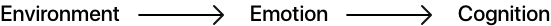
\includegraphics[width=200px]{graphics/relation1.png}
\end{center}
 
There is strong evidence of the surrounding environment having an influence on emotion \cite{Johnson2000, Arockiam2013, Bertamini2013}. This includes, for example, an e-learning system on the screen in front of the learner. In a similar fashion several studies have shown a correlation between emotion and cognition (Section \ref{sec:emotion-cognition}).

\begin{center}
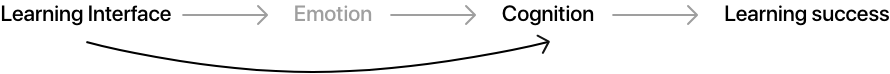
\includegraphics[width=300px]{graphics/relation2.png}
\end{center}

There is a logical argument of the existence of a transitive relation between these parameters, which could confirm the dependency of the edge variables. 
I.e. exposure to several interfaces each with a different emotional charge during an on-line lesson should lead to a difference in performance when working on the same task.
Insufficient research confirming this connection and explaining the effects has been published yet. 

In this paper I would like to explore to which extent the final parameter "learning success" can be influenced with the limited surface of contact that can be addressed through a learning interface on the screen.
	
		
	\subsection{Research basis} \label{sec:research}
	
	\toDo{about 10 pages of research}
	
	Information architecture and display types play an important role in learning comprehension, attention and learning success. \cite{McCrudden2017} describe the effects of different types of visual display on cognitive processing. They highlight the important aspects of visual guidelines, the basics of human understanding and  memory, as well a way to quantify those under processing efficiency. One of their conclusions is that "displays should be designed to support the selection of important information" \cite[p.633]{McCrudden2017}
	
	There is, however, a case to be made with respect to the same visual display that can be put forth in front of participants under differentiating emotional states. There is strong evidence that emotions play a role in information processing and, as a consequence, can have an effect on the resulting performance. Section \ref{sec:emotion-cognition} discusses closer existing research supporting a connection between emotion and cognition.
	
	Evidence also suggests that specific emotion can be caused through the use of emotional design features. Section \ref{sec:emotional-design-features} proposes a set of general rules for emotional design based on previous research.
	
	A recent study \cite{Haaranen2015} suggests that wrong choice of emotional design patterns can yield contra-productive results. It reports lover concentrations levels in the experiment group compared to control group using abstract graphics when learning object-oriented programming (OOP). Due to their choice of presentation and the topic of learning, the material has not been perceived as serious and lead to lower self-reported concentration levels.
		
		\subsubsection{Emotion theory} \label{sec:emotion-theory}
		
		To understand how emotion acts as a mediator to e-learning and learning in general it is important to see what emotion is and what causes it.
		
		From a biological perspective \textbf{emotion} is a collection of responses triggered from parts of the brain to the body or other parts of the brain. A series of such responses results in an \textit{emotional state} and is defined by changes within the body. \cite{Damasio1998}
	
		Emotion is caused by various internal and external events. Internal events can be immune activity or hormone changes. External events - observed or felt in the outside world - contribute additionally to internal ones. People have do direct access to the causal connections of emotions and little to no control of them. One can undergo a change of emotion without knowing why. \cite{Russell2003}
		
		Russell proposes that at the base of any emotion the experienced states are either good or bad, energized or enervated. As such these are the two "core affects" that govern our perception, behavior and cognition. \cite{Russell2003}. 
		
		There are individual differences of average levels of core affect and its responsiveness to stimuli due to the genetic differences. \cite{Russell2003}
		
		From the end of the 19th century and up until early 21st century, psychological research papers proposed a range models for representing emotion . Those can be grouped into categorical and dimensional models. The former classify emotions into a set of specific discrete labels and often include emotions such as 'anger', 'disgust', 'fear', 'joy', 'sadness' and 'surprise'. The question of on how many and which types of emotions exist is being argued among researchers. 
		Labels and central emotions can differentiate depending on the domain, whereas an education model might suggest those, that are most common in this context: 'boredom', 'confusion', 'joy', 'flow', and 'frustration'.
		
		Dimensional models, conversely, describe affect on a set of dimensions. Each concrete emotion is assigned to a location in this space. A dimensional model provides a better framework for measuring and comparing emotional states to categorical \cite{SreejaPSMahalakshmi2017}, \cite{Harley2016}.
%		Often the dimensions are of \textit{valence}, \textit{arousal}, and \textit{dominance}.
		
		A popular approach is the "Circumplex Model of Affect" \cite{Russell1980}, where emotions are summarized and laid out in a two-dimensional space. The horizontal axis describing the "pleasure" (further used as valence) dimension. The vertical axis - the arousal dimension. These two dimensions are treated as independent.
		
		\begin{figure}[t]
			\begin{center}
				
\includegraphics[width=150px]{graphics/Valence-Arousal-Model-0.png}
				\caption{Valence Arousal Model. Figure adapted from \cite{Song2013} \label{fig:valence_arousal_model}}
				
			\end{center}
		\end{figure}
	
		Assumptions in the current paper are largely based upon the "Circumplex Model". I classify possible emotional states into four quadrants which are mutually discrete. To simplify, they are be labeled for further reference as shown in figure \ref{fig:valence_arousal_model}):
		\begin{enumerate}
			\item[Q1:] Angry 	(Quadrant 1)
			\item[Q2:] Happy 	(Quadrant 2)
			\item[Q3:] Sad 		(Quadrant 3)
			\item[Q4:] Relaxed 	(Quadrant 4)
		\end{enumerate}
		
		These labels are used interchangeably throughout the paper.
		
		While there is a general consensus among researchers that arousal and valence are critical features of emotions \cite{Harley2016}, some sources suggest a third dimension of "dominance" to be added to the representation to form the PAD (Pleasure, Arousal, Dominance) Model. Dominance dimension ranges from \textit{controlling and dominant} to \textit{controlled/submissive}. For example, fear and anger are very similar on the pleasure and arousal scales. On the dominance scale anger is a dominant emotion, while fear is submissive \cite{Mehrabian1974}.
		This study does not consider the dominance dimension in the analysis framework.
		
		
		\subsubsection{Visual interface and emotion}
		
		\cite{Desmet2007} demonstrates in their research that physical objects can cause significant emotional response and that modifying design attributes can successfully contribute to creating of desired response.
		Both physical objects and digital visuals are, in essence, interfaces. As corroborated by emotion theory any interface we acknowledge and, especially interact with can cause an emotional response. 
		
		Nowadays, user's attention spans are increasingly short and distractions are more common than ever. With the advent of Web 2.0 and the increasing speed or computers and consumer oriented digital products we are accustomed to quick, precise responses. Users grant low tolerance to shortcomings in an interface. Abundance of alternatives leads to consumers choosing the product that can cause the most pleasant emotional affect.
		
 		Digital interfaces are extremely flexible to experimentation and modification at a relatively low cost, compared to conventional physical products.
 		The industry  experimentation, research, and improvements in user interface practices, especially when it comes to emotions.
		%%%%%%%%%%%%%%%%%%%%%
		
		
		%\paragraph{Literature review}
		
		A paper by L. Arockiam et al \cite{Arockiam2013} suggests that, based on previous research and their own findings, optimal user interface can be achieved when you add a person's personality traits into consideration. This finding could mean a mediating effect of participant preference on the universality of interface attributes aimed at evoking high arousal. 
		
		Current study aims to find a general set of attributes that should evoke high arousal and positive valence.
		
		\paragraph{Color}
		
		A 1996 research paper \cite{Pert1996} provides a wide overview of literature and delivers important insight about color, citing an array of previous research. The following paragraphs on color reference \cite{Pert1996}, unless otherwise stated. The paper provides a categorization of color effect on a person into three distinct types: physiological, psychological, and learning related. As asserted in \ref{sec:emotion-theory} and \ref{sec:emotion-cognition} all of these can be understood as interrelated, as both physiological and psychological processes take an effect on emotion and learning.
						
		Nevertheless, following the distinction made by Pert et al., a \textit{physiological effect}, in particular - arousal is shown in \cite{Wilson1966} with reported higher galvanic skin response (GSR) measurements for red color as opposed to green. 
		Nourse and Welsh (1971) reported higher GSR for violet than green.
		Jacobs and Hustmyer (1974) found that red was significantly more arousing than yellow or blue, 
		Jacobs and Suess (1975), although, found that red and yellow resulted in a higher anxiety state scores than blue or green.
		
		Overall \cite{Pert1996} suggests that spectral extremes, like red and violet, cause greater arousal than colors in the middle of the spectrum.
		
		Under \textit{psychological effects} of color Pert analyses preference, meaning and perceived harmony between colors.
		
		A 1941 study \cite{Eysenck1941} ranks preferences of colors presented on colored pieces of paper. 
		The order of preference is: 1 - blue, 2 - red, 3 - green, 4 - violet, 5 - orange, 6 - yellow. Earlier studies conducted among 21,060 subjects conclude the same average selection of color preference. Important trait of these results is that the order is observed to be the same for all races and for both men and women. A single difference is manifested at the far end of the preference scale, where men choose orange over yellow, while women choose yellow over orange.
		
		In 1963 \cite{burnham1963color} affirms the lack of significant differences between men and women or between different races on color preference.
		
		These findings are expanded in a study on color and emotion \cite{Valdez1994}, where the results show that men and women have a similar emotional reaction to variations in saturation and brightness. A slight consistently stronger emotional response is recorded by women compared than men. This could suggest that women are more influenced by visual stimuli.
		
		Schaie (1966) reports, somewhat contrary to previous findings, that color preferences relate to personality of an individual and can vary. A stronger preference of cooler colors by introverts and warmer colors by extroverts is reported by C. Robinson (1975).
		
		A study among school children between first and twelfth grade finds that girls of all ages prefer brighter colors as compared to boys (Child, et al., 1968). This finding is of limited relevance and may find limited degree of comparability to adults, as it focuses on children. Winn and Everett (1979) states that color in pictures has greater impact on meaning among young people.
				
		In a study by Adams and Osgood in 1973 conducted across 23 different cultures a general preference for cool colors (blue/green) compared to warm colors (red/yellow) has been established. Pert asserts that cool colors tend to rate higher on average across cultures, ages and individual characteristics.
		
		Among the suggested uses of color Pert suggests using a color like "highly saturated red and violet to attract attention and to create an emotional response" \cite{Pert1996}, and to consider color associated meanings i.e. red means stop, the meanings attributed to colors can also differentiate among cultures.
		
%		An extensive study on effects of hue, saturation and brightness of color of emotional 
		
		While colors at the ends of the spectrum cause greater arousal, those in the middle of the spectrum, like green and cyan, are reported to be best for emphasis. \cite{Pert1996}. The paper suggests that red, having an arousal effect could potentially be more effective than middle-spectrum colors to attract and hold attention. Brightness of color is suggested to affect the mood attributed to that color more than it's hue.

		A 1994 study \cite{Valdez1994} of effect of color on emotions asserts that previous studies have not accounted for compounding effects of hue, brightness and saturation when analyzing color effects and aims to separate these factors. Emotions in this study are rated (similarly to approach in this study with one added dimension) on three scales: arousal, pleasure and dominance. They completed three experiments.
		The first experiment involved two hundred and fifty subjects and analyzed emotional impact of color saturation and brightness. The experiment concluded a highly significant trend that arousal is increased linearly with color saturation and decreased with color brightness up to value 43 of the Munsell brightness scale. On higher levels arousal increased slightly. Pleasure is a positive function of both brightness and saturation, while being influenced more strongly by brightness, than saturation. In other words highly saturated, bright colors are most pleasurable.
		The second experiment had 121 people rate different hues. The experiment found consistent support to the hypothesis that hue exerts effect on the pleasure dimension. In this study blue, blue-green, green, purple-blue, red-purple, and purple	were found the most pleasant hues. Results for the arousal and dominance dimensions were far weaker.
		The third experiment analyzed achromatic colors. Here, arousal response was strongest for black, diminished for three successive grays, but then increased to an intermediate value for white. Black was rated as least pleasant, grays intermediately pleasant, while white was the most pleasant. \cite{Valdez1994} 
		
		A recent study by \cite{Wilms2018} takes another look at the same problem. Compared to Valdez et. al. conducted in 1994 where colors are presented on printed cards, this 2018 study presents research in connection with an LED screen. Sixty two participants viewed each color for thirty seconds and rated their emotional state. This paper limits the scale to valence and arousal values, bypassing dominance. Colors were also limited to 3 variations of each dimension (hue, saturation, brightness). The study confirms only limited differences of color perception between genders. Further the study shows that hue and saturation have significant effect on arousal ratings, where high saturated red colors show highest arousal. Saturated and bright colors cause significantly stronger skin conductance responses (SCR), high chroma colors cause short-term heart rate acceleration. Emotional effect of colors is shown to be determined by all 3 colors dimensions - hue, saturation, brightness (HSB) as well as their interactions. This, confirms several findings presented earlier in \cite{Valdez1994}. \cite{Wilms2018} note that although the findings corroborate previous studies on the topic, studies that have taken emotional pictures report much higher correlations between reported values and SCR measurements.
				
		\cite{Zielinski2016} compares self-rated judgments and SCR of users when presented with color stimuli. Results show that only saturation (and not hue or brightness) has an effect on SCR levels. Significant correlation is reported between self-ratings and SCR. Paper suggests that "more saturated stimuli are better in capturing attention".
		
		Overall, there is strong evidence of colors having an direct impact on emotions, both on psychological and on physiological levels, although colors by themselves are less impactful than images or other emotional stimuli that possess additional semantic meaning.
		
		
		\paragraph{Color and learning} Below I summarize studies that discuss color use in learning and cognition environments (unless stated otherwise this paragraph uses as source the summary paper \cite{Pert1996}).
		
		A 1960 paper (Kanner and Rosenstein, 1960) studies color-effectiveness at Fort Monmouth in typical army training procedure. 11 video lessons are used with monochrome and colored versions of television. No significant differences are found in learning between both. In 1961, in a similar study of effects on learning with colored versus black-and-white television, no significant differences are reported \cite{Pert1996}.
		However, historical context is important to note here, as during this time television resolution and color reproduction has not been as vivid and realistic as nowadays. Stronger, more saturated colors are found to be more potent in causing emotional affect \cite{Valdez1994}.
		
		Several studies agree that "colored materials are preferred by learners", can promote acceptance of a learning medium and can influence affective meaning of the illustrations \cite[p.25]{Pert1996}.
		
%				(so far black and white and color has not yielded any significant difference in learning)
		Color can be used as an attention getting device. In a research study on color coding, Lamberski and Dwyer (1983) conclude that color, when used in this way, can provide measurable effects on learning, that cannot be accounted for by words and labels. 
%		\cite{Pert1996}
		Search tasks can be more efficient, measured by search time, when color is used for color-coding, with up to five colors. Additionally color is found to be useful in grouping information. \cite{Pert1996}
		
		Retention can be improved with color when it adds additional informational value or visual complexity to the object being displayed. As such, color versions result in higher recognition memory scores in immediate recognition memory tests and under some conditions (non-realistic color use) for delayed tests. A 1981 study suggests that colored line drawings and especially those on a black background have significantly higher recognition scores compared to uncolored line drawings \cite{Pert1996}.
		
		\cite{Pert1996} concludes that "the key factor relating to color and cognitive learning seems to be that it is of value when it emphasizes relevant cues, is used as a coding device, or when it is a part of the content to be learned".
		
		A 1970 study suggests that when presented with video material (for example te "Grey Cup" football game) participants react more emotionally to the color versions, compared to more detail-oriented when watching the monochrome version.	The study concludes that color creates emotional effects that detract from attention to details.
		
		Random use of color is not associated to increased learning, although evidence shows that color can increase retention \cite{Pert1996}.

		In a more recent study on effects of emotional design in 2014 (\cite{Plass2014}) participants are asked to learn material on immunization. The lesson is split by groups where one group sees colored version and another - monochrome. The analysis shows that colors used in the emotional design in this study increase comprehension (specific definitions of terms), but do not induce positive emotions and do not increase knowledge transfer (abstraction to general ideas). Moreover, transfer is reported to be lower under certain conditions when using color design, drawing a conclusion that color can be detrimental to learning.
				
		In summary, conflicting accounts are found as to the effect of color on emotions. Some evidence suggests that certain color values, that are similarly appraised across ages, genders and cultures, can be derived. The range of these can be fairly limited as research found that color perception differentiates on all aforementioned levels and, additionally, can vary due to personal preference. Past research often fails to provide exact color values including hue, brightness, saturation and luminescence of the colors used in the analysis. More research is required in this domain to provide a more clear picture. 
%		Cautious use of color for eliciting emotion is advised.
		
%		\cite{Valdez1994} - effects of color on emotions
%		\cite{Pert1996} - Color Research and Its Application to the Design of Instructional Materials
		
%		\cite{Tekirdag2015} - The Effect of Colour on Human Body and Psychology - bad
%		\cite{Swasty2017} - Does Color Matter on Web User Interface Design? - this is bullshirt
%		\cite{Plass2014} - Emotional design in multimedia learning: Effects of shape and color on affect and learning
		
		\paragraph{Shapes}
		
		A study \cite{Larson2007} on detection and perception of geometric shapes assesses the factor of dislike between three shapes: downward-pointing triangles, upward-pointing triangles and circles. Circles are significantly the least disliked shape, with upward triangles and downward triangles taking the second and third place respectively. Differences between all three groups are significant. Other findings show that on a matrix of shapes, where one cell contains a different shape, the speed and accuracy of detection of the divergent shape is higher when the shape is the downward V compared to the other shapes tested. The research explains the findings as rooted in the threat detection of the human brain, which is highly efficient.
		
		A later study from \cite{Larson2012} further expands the research with a wider range of geometric forms. The research concludes that downward-pointing V’s are perceived as threatening and curvilinear forms are perceived as pleasant.
		
%		\cite{Larson2007} - The Shape of Threat: Simple Geometric Forms Evoke Rapid and Sustained Capture of Attention.
				
%		\cite{Larson2012} - Simple geometric shapes are implicitly associated with affective value
		
		In the study by \cite{Plass2014} researchers compare use of two types of shapes for representing objects in the learning materials. One of the versions uses square shapes, the other round face-like shapes. The study suggests that, "designers aiming to enhance learners’ comprehension of the material can use [...] round face-like shapes rather than square, non-face like shapes in their designs" \cite{Plass2014}. The findings show evidence, that round shapes impact positively both transfer and comprehension of learning material.
		
		A related study \cite{Park2015} suggests that anthropomorphisms as such (see figure \ref{fig:anthropomorphisms}) to be ineffective in inducing positive emotions, but effective in arousing attention.
		
		Face-like elements in online interaction are discussed in related studies.
		For instance \cite{Walther2001} analyzes the "Impacts of Emoticons on Message Interpretation in Computer-Mediated Communication" and observes, that for positive messaging positive emoticons (in textual representation) improve the happiness perception rating for that message.  
		
		Emoticons provide computer based communication with a more social and interactive experience. In an e-learning environment emoticons can enhance teaching presence. \cite{Dunlap2016}
		Emoticons are perceived in the brain in a very similar way to real human face expressions. \cite{Churches2014}
		
		\subsubsection{Emotion and cognition} \label{sec:emotion-cognition}
		
		Even through there has not been yet an exact formula developed of the relationship between emotion and cognition, studies agree in their general conclusions, that emotion displays a significant impact on cognitive processes \cite{Sakaki2012, Leutner2014}
		
		A 1992 study \cite{Bradley1992} on emotional pictures and memory concludes that pictures rated as highly arousing are remembered better than low-arousal stimuli.
		
		A 2004 cognitive neuroscience study \cite{Dolcos2004} scanned participants brain activity, while rating emotional pictures. The study makes several relevant conclusions. First, that different parts of the brain show stronger activity when exposed to positive compared to negative stimuli. Second, that high arousal stimuli lead to greater successful encoding activity, or - rate of recall, than neutral stimuli. 
		
		In other words, brain response is different for arousing stimuli of positive valence compared to negative valence. Furthermore memory is mediated, in part by both - valence and arousal levels. It provides basis to the assumption that variation on both dimensions is necessary to adequately reflect effects within e-learning context. Study design in \ref{sec:study-design} depends heavily on this assumption.	
				
		A study on the influence of music, particularly Mozart, on the performance showed that participants perform better on a spatial ability task after listening to Mozart. The analysis shows that the effects correlate with the change in mood suggesting that the "Mozart effect" is explained by the underlying emotional affect caused by music \cite{Thompson2001}.

		In discussion of the findings \cite{Jefferies2008} state that sadness (low arousal, low valence) is associated with attention to the details, while joy is linked to a more creative, global thinking manner. Important to note that change of performance is not evident across all tasks discussed and therefore lead to suggestion, that effect of mood does not generally improve or impair performance, but rather specific cognitive processes. It also notes the possibility that performance is not linked to any level of core emotional dimension, but rather a combination of those leading to an emotional state.
%		\cite{Jefferies2008} Emotional Valence and Arousal Interact in Attentional Control
		
		\cite{Park2015} reports that learners in a positive emotional state have better learning outcomes in comprehension and transfer tests and show longer fixation on the relevant information of the learning environment.
		
		A study in 2015 analyses the learning success of 206 undergraduate students with a 40 second animation after preconditioning them to one of four groups: positive-calm, positive-arousing, negative-calm, negative-arousing. Materials are presented either as written text or voice narration. The results show that arousing groups outperformed calm groups on a recall test, but only in the written text condition. The authors conclude, that the results imply, that the arousing emotional state has the potential to enhance multimedia learning. \cite{Chung2015}

%		OMITTED:
%		\cite{Sternberg2010} Emotion and E-Learning
%		\cite{Leutner2014} Motivation and emotion as mediators in multimedia learning
		
		\paragraph{Emotional design and Learning} 
		
		Some recent studies approach the effects of emotional design in connection with learning achievement. A 2014 study takes a similar approach to current study, by having two preconditioning sequences (neural and positive) and two design versions. Emotional design is applied to learning materials directly in the form of shapes (rounded, face-like features) and colors (color vs black-and-white).
		
		The study shows a range of findings. Positive emotional design causes positive affect which is sustained over the learning session. Mood induction through positive preconditioning also causes positive affect successfully, although it induces a different kind of emotions on the learner, which suggests that the two ways to induce emotions work in different ways. 
		Emotional design is found to decrease perception of task difficulty and increase motivation.
		
		The study also finds that positive emotional state induced (internally) through the emotional design of the learning materials, leads participants to perform better on the comprehension test (asking for specific definitions of terms), but does not increase transfer (asking learners to apply knowledge by answering questions related to the general ideas, not to specific details). External (cartoon conditioning) induction, contrarily, enhances transfer, but not comprehension.
		The results are reported to be only partially consistent with an earlier study conducted by the researchers and similar in design. The previous study has suggested that both comprehension and transfer increase with emotional design \cite{Plass2014, Plass2016}.
		
		A similar approach with emotional design features applied to materials is considered by \cite{Mayer2014}. Students are presented with a lesson in one of the two versions: control or enhanced (see figure \ref{fig:benefits-bio-lesson}). In the control group, the graphics consist of simple black-and-white drawings. In the enhanced group, the graphics use anthropomorphic feature and use color. The study shows that the enhanced group performs better, than the control group on a subsequent learning test. A similar conclusion is made in \cite{Le2018}. Additionally \cite{Le2018} outlines a difference in physiological response to emotional design with a stronger decrease of heart rate variability compared to the control group
%				The effect of emotional design on mental effort investment was investigated
%Results validate incorporating positive emotion graphics in multimedia instructions.
%Stronger decrease of HF HRV were observed in positive design group.
		
		Other studies show modification of the environment without directly influencing the learning material.
		
		\cite{Lee2014} discusses the effects of various presentation methods of multimedia instructional on students’ learning outcomes. The paper compares a regular "PowerPoint presentation" with the one guided by a human-like animated character and one guided by a monster-like animated character (shown in figure \ref{fig:theeffectsofmultimediainstructionalmaterials}). The authors suggest that human-like animated character method outperforms the other methods in regard to the emotional response of students. Further, socialness perceptions, arousal, pleasure, flow experience, and learning motivation can all affect students’ learning outcomes. It is advised to consider students’ previous learning habits when designing instructional materials, and to convey a sense of professionalism (encouraging students to invest time in learning).
	
		\cite{Heidig2015} uses the concepts from web design to extract how emotional design influences learning. The study analyses several types of color combinations around e-learning materials and their effect on motivation and learning. Differences in aesthetics or usability did not affect learners’ emotional states as expected across groups in this study. However, participants perceived aesthetics and perceived usability significantly predict participant's perceived emotional state. The paper concludes that participants response to design features is highly dependent on the expectation of the user and their learning situation (time pressure, intrinsic motivation). Outcome of the study includes that emotional state during learning has a minor impact on learning outcomes but a larger impact on learners’ intrinsic motivation.
		
		Positive effects of emotional design can be negated when overused or used improperly. According to \cite{Chang2014} previous studies suggest the effect of \textit{seductive details} is detrimental to learning success. The study finds that seductive sentences force attentional allocation to themselves and hinder information retrieval. Seductive pictures, on the other hand, do not result in strong effects on the learner, the study suggests.
		
%		\cite{Chang2014} Effects of seductive details evidenced by gaze duration.
%		(Lehman et al., 2007) showed that the presence of sentences with seductive details had a significant negative effect on the amount of time the participants spent. According to the recall analysis, those participants who read the baseline passage (i.e., no seductive sentences) were significantly more likely to recall important information than those who read the seductive passage reading baseline sentences.
		
		\cite{Brom2018} How effective is emotional design? A meta-analysis on facial anthropomorphisms and pleasant colors during multimedia learning.
		
		Anthropomorphisms and pleasant colors should enhance multimedia learning
		Anthropomorphisms/colors consistently increased learning outcomes
		Their effects on affective-motivational states were weaker and less robust.
		Anthropomorphisms/colors are beneficial, but the mechanism is unclear.
		
		\cite{Uzun2018} Exploring the effect of using different levels of emotional design features in multimedia science learning
		
% 		Because working memory can only hold a limited amount of information (Baddeley, 1986, Cowan, 2001), processing of multimedia information is performed under these memory constraints \cite{Plass2016}
	
	\subsection{Hypotheses} \label{sec:hypothesis}
	
		To validate if there is a difference between emotional responses to the two different design approaches and consequently check if any design differences lead to a different performance of learning sessions two hypotheses are proposed:
	
		\paragraph{Hypothesis 1.} H$_{0}$: Two different proposed interfaces do not result in a significant difference in emotional response.
		
		\paragraph{Hypothesis 2.} H$_{0}$: Performance of participants on memory and creativity tasks, as measured by selected study design parameters, during the experiment is equal using interface 1 compared to using interface 0.

\section{Approach and Methods}

To facilitate the study I make assumptions about the medium in which e-learning is usually conducted. Based on previous research (\ref{sec:research}) I define study design parameters and a set of target variables that are measured and evaluated.

	\subsection{Medium}
	
	The study is to be conducted online under a "real-life" scenario. This means, that the experiment is to be run in a browser-capable web-application runnable on modern personal computers. Like most e-learning software the  application used in the study is browser-based and usually used in a user's home or public venue.
	
	\subsection{Study design} \label{sec:study-design}
	
	Goal of the current study is to determine emotional response difference to provided emotional design implementation (Interface 1) compared to the control group that is provided with a stricter desaturated design (Interface 0). Differences include use of color, shapes, language, font style, interaction responsiveness, animation. The similarities or - constant variables - across both interfaces include any accessibility features and general usability heuristics, such as contrast ratio level, size and placement of elements on a screen. Further details of the emotional design aspects, that are included in the current implementation are shown in section \ref{sec:emotional-design-features}
	
	Participants of the study are not informed about the existence of another interface as a variable but rather only made aware about being emotionally influenced by preconditioning and that their performance during the experiment is being measured. Abundance of timers throughout the test highlight the time sensitivity of the tasks to the participant. This is a \textit{between-subject} experiment with each combination of four preconditioning and two interface version is tested once for each participant
	
	The experiment can be outlined and split into following steps:
	
	\begin{enumerate}
		
		\item[0.] \textbf{Clustering:} Each participant is assigned an interface version (one of two) and the preconditioning group (one of four) at random before first load of the application.
		
		\item \textbf{Emotional report [SAM1]:} A short emotional self-reporting questionnaire (SAM \ref{sec:selfeval}) is used to acquire initial valence and arousal ratings
		
		\item \textbf{Preconditioning:} Each participant is shown a set of emotional images and preconditioned to be in one of 4 states:
			\textbf{1}: Positive valence / high arousal;
			\textbf{2}: Negative valence / high arousal;
			\textbf{3}: Positive valence / low arousal;
			\textbf{4}: Negative valence / low arousal;
			
		Choice of stimuli and their presentation is described further in chapter \ref{sec:preconditioning}
			
		\item \textbf{Emotional report [SAM2]:} A second emotional self-reporting questionnaire (SAM \ref{sec:selfeval}) to validate, whether preconditioning has had a sufficient and expected effect on the participant.
		
		\item \textbf{Experiment 1:} Slightly modified classic memory game. The participant is presented with a grid of tiles, each tile containing an image. During 10 seconds at the beginning of the experiment all tiles are open to allow to memorize the images. After which all images are hidden. Only 2 tiles can be opened at any one time. Once both tiles of the same image are open they are marked as solved. The goal is to solve all tiles. Detailed description in section \ref{sec:memory}
		
		\item \textbf{Experiment 2:} Remote Associates Test (RAT). A generalized creativity test developed by Mednick \cite{Mednick1962} in 1962. Each participant is presented with a number of word sets. Each set consists of 3 words that are shown to the participant and one target word that is hidden from the them. The target word is semantically connected to all 3 visible words. Detailed description in section \ref{sec:creativity}
		
		\item \textbf{Emotional report [SAM3]:} A third emotional self-reporting questionnaire (SAM \ref{sec:selfeval}) is used to establish, whether and which effect tasks and interface have had on the participant's emotion.
		
		\item \textbf{Demographic data:} Final step adds additional personal context data for each participant through a questionnaire to complement data analysis (discussed in \ref{sec:demographics}).
		
	\end{enumerate}
	
	\subsection{Preconditioning sequences} \label{sec:preconditioning}
	
	\paragraph{Finding a preconditioning sequence}
To facilitate emotional conditioning I selected a specialized sequence containing images with a corresponding emotional charge.
Each sequence contains 21 to 39 \todo{more precise} images with each displayed for about 5 seconds.

Each subject is assigned one of four preconditioning sequences. Each sequence is aimed to condition the subject into one of the 4 quadrants, described though a valence-arousal emotional model. To simplify we will label (\ref{fig:valence_arousal_model}) them as:
\begin{enumerate}
	\item Angry (Quadrant 1)
	\item Happy (Quadrant 2)
	\item Sad (Quadrant 3)
	\item Relaxed (Quadrant 4)
\end{enumerate}


\begin{figure}
\begin{center}
	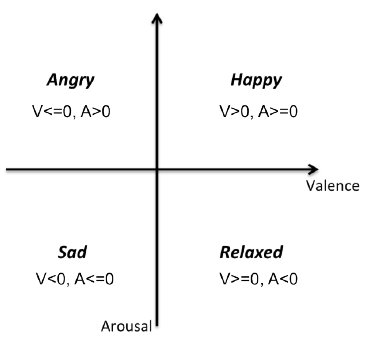
\includegraphics[width=150px]{graphics/Valence-Arousal-model-showing-the-quadrants-of-the-four-emotion-tags-used-in-this_W640.jpg}
	\caption{Valence Arousal Model \cite{Song2013} \label{fig:valence_arousal_model}}
	
\end{center}
\end{figure}

There are several emotional image data-sets available for academic purposes such as GAPED \cite{Dan-Glauser2011}, OASIS \cite{Kurdi2017}, IAPS \cite{Lang1997} and NAPS \cite{Marchewka2014}. While NAPS is offering the highest realism and quality of images, the range images seems to cover "sad" and "happy" to a less pronounced degree. In general, strong negative valence values are accompanied with high arousal values across all analyzed data-sets. Causing sadness is a challenging task. In current preconditioning sequences I am using the \textbf{OASIS} database. It has relatively wide spread of emotions compared to other sets.

Keeping in mind the need for a clear separation between groups in terms of their emotional state into account, I limited emotional images to moderately strong stimuli values, thus avoiding extreme reactions and unrealistic emotional states. It can be assumed that in most cases, people who attend e-learning lessons will have moderate levels of emotional charge. It is important to note that quadrant 1 - angry and quadrant 2 - happy has a more pronounced representation in emotional databases due to an easier and more prevalent stimuli availability. As such quadrant 1 and quadrant 2 have stronger stimuli compared to quadrant 3 and 4. It is expected that there will be a significant difference between emotion ratings of participants across these groups.

It is understood that the e-learning interface under real conditions will only cause mild-to-moderate changes to a mood.


\begin{figure}
	\centering
	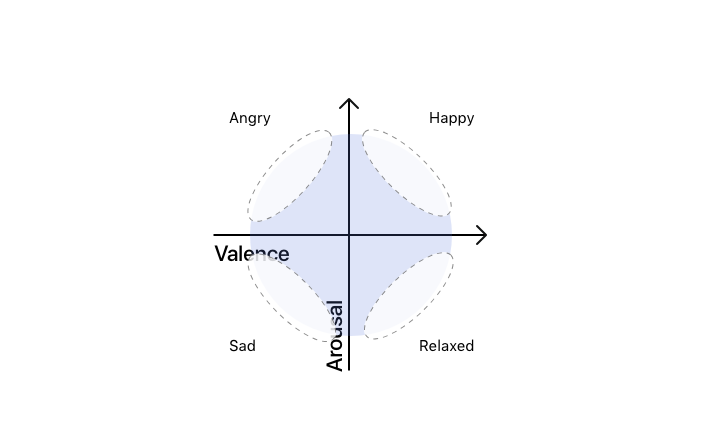
\includegraphics[width=0.7\linewidth]{graphics/Valence-Arousal-Model-1.png}
	\caption{Focus levels of emotional states on valence arousal model}
	\label{fig:valence-arousal-model-2}
\end{figure}

Illustration \ref{fig:valence-arousal-model-2} highlights with dashed outline areas the target arousal and valence values

	
	\subsection{Emotional Design Features} \label{sec:emotional-design-features}

	Studies shown in section \ref{sec:research} strongly suggest a connection between user interface and learning performance. They analyze performance and presentation based on concrete learning content examples. In present study I attempt to generalize the findings to a more universal set of guidelines that is not specific to certain content and could be applied to any e-learning topic.
	
	Emotional design has a limited surface area of possible modifications due to the focus being on the content. Under real conditions it can be expected that the e-learning interface will cause mild-to-moderate changes to affect. In part, those changes are also attributed to the task at hand, rather than the emotional design attributes.
	
	\cite{Brom2018}: Anthropomorphisms/colors consistently increased learning outcomes.
	
	\cite{Le2018}: Compared to the participants in the neutral design group, the participants in the positive emotional design group performed better on a subsequent retention test
	
	\cite{Uzun2018} Exploring the effect of using different levels of emotional design features in multimedia science learning


	\clearpage

\paragraph{Developing a high performing interface}

There is a multitude of studies that analyze user interface design and user emotion. In following I will summarize them in respect to UI features tailored towards high performance

\paragraph{Literature review}

A paper by L. Arockiam et al \cite{Arockiam2013} describes that, based on previous research and their own findings optimal ui can be achieved based on a person's personality traits. We will limit ourselves to a universal set of changes that should evoke high arousal, positive valence and therefore have an effect on learning outcome, rather than look for their preference. Nevertheless it is worth mentioning...

Color - PHYSIOLOGICAL

Wilson (1966) reported higher GSR measurements for red as opposed to green, and Nourse and Welsh (1971) reported higher GSR readings for violet than green. Using 24 male college students as subjects and saturated samples of red, yellow, green, and blue as stimulus materials, Jacobs and Hustmyer (1974) found that red was significantly more arousing than either yellow or blue, and green more than blue. Using 40 undergraduate students as subjects, Jacobs and Suess (1975) found that red and yellow resulted in higher anxiety state scores than blue or green when measured by the StateTrait Anxiety Inventory. Bloomer (1976) also reported that red increases heart rate. There appears to be some evidence that spectral extremes, especially red, cause greater arousal than mid-spectral colors. This may relate to the fact that wavelengths at the extremes of the spectrum, such as red and violet, focus at different points in the eye than wavelengths at the middle of the spectrum. \cite{Pert1996}

Color - PSYCHOLOGICAL

The selected order of preference was: (1) blue, (2) red, (3) green, (4) violet, (5) orange, (6) yellow. This selection agreed with the average rankings of color preference among 21,060 subjects reported in earlier investigations. The order was the same for all races and for men and women with one exception. Men chose orange over yellow whereas women chose yellow over orange. \cite{Pert1996}

no significant differ- ences between men and women or between subjects of different races.\cite{Pert1996}

girls of all ages preferred higher value, brighter, colors as compared to boys (Child, et al., 1968) \cite{Pert1996} (study among school age children from 1 to 12 grade)

Results on the evaluation scale supported the general preference for cool colors(bl~e and green) as compared with warm colors(red and yellow) and agree with previous findings by Adams and Osgood (1973) that red is a potent color while gray and black have low potency. \cite{Pert1996}

In a color-effectiveness study conducted at Fort Monmouth, typical army training procedures were used with 11 different television lessons (Kanner and Rosenstein, 1960). No significant
differences were found in learning between
monochrome and colored versions \cite{Pert1996}

Schaie (1966) pointed out that color prefer-
ences vary from individual to individual and relate to personality. \cite{Pert1996}

(so far black and white and color has not yielded any significant difference in learning) but "colored mate- rials are preferred by learners." \cite{Pert1996}

1972: those who viewed colored transparencies had had a more positive attitude toward transparencies than \cite{Pert1996}

In a research study on color coding, Lamberski and Dwyer (1983) concluded that color is an attention-getting device that can provide measurable effects on learning that cannot be accounted for by words and labels. \cite{Pert1996}

Search Tasks: 
gain in efficiency, indicated by decreased search time, with codes of up to five colors \cite{Pert1996}

Color was found to be useful in grouping information

color versions resulted in higher recognition- memory scores (immediate recognition memory test)\cite{Pert1996}

as the variable of visual complexity increases, so does the degree of recall. (Berry (1991a)) \cite{Pert1996}

The key factor relating to color and cogni-
tive learning seems to be that it is of value when it emphasizes relevant cues, is used as a coding device, or when it is a part of the con- tent to be learned (Dwyer and Lamberski, 1982- 83; Levie, 1973; Pruisner, 1993; Wedell \& Alden, 1973). \cite{Pert1996}

Non-objective Measures

(Scanlon, 1970). Scanlon suggests that the color versions (Grey Cup football game) create emotional effects that detract from attention to details.







Colors at the ends of the spectrum, red and
violet, seem to result in greater arousal, and
colors in the middle of the spectrum, yellow,
green, cyan, seem to be best for discriminating
detail. \cite{Pert1996}
	
	\subsubsection{Developing an "optimized" interface}
	
	\toDo{write which interface elements are considered}
	
	\begin{itemize}
		\item Roundness of shapes vs corners
		\item warm colors vs cold colors
		\item smiling faces vs "X"
		\item responsiveness of ui (hover states and movements)
		\item more animations (for spacial more realistic feeling) such as tiles
		\item font family (rounded and edgy)
		\item use of wording, tone of voice and language \cite{Hancock2007}
	\end{itemize}

	Memory experiment page shows a smiling face icon. On-site questionnaire is conducted during creation of the experiment to determine an icon which is portraying the strongest "happiness" emotion. A previous iteration also contained a female version of the image. It has been excluded to avoid an effect of gender bias. Figure \ref{fig:smiling-icons} shows the 3 versions tested. Version 3 is finally used in the live test run.
	
	\begin{figure}[h]
		\centering
		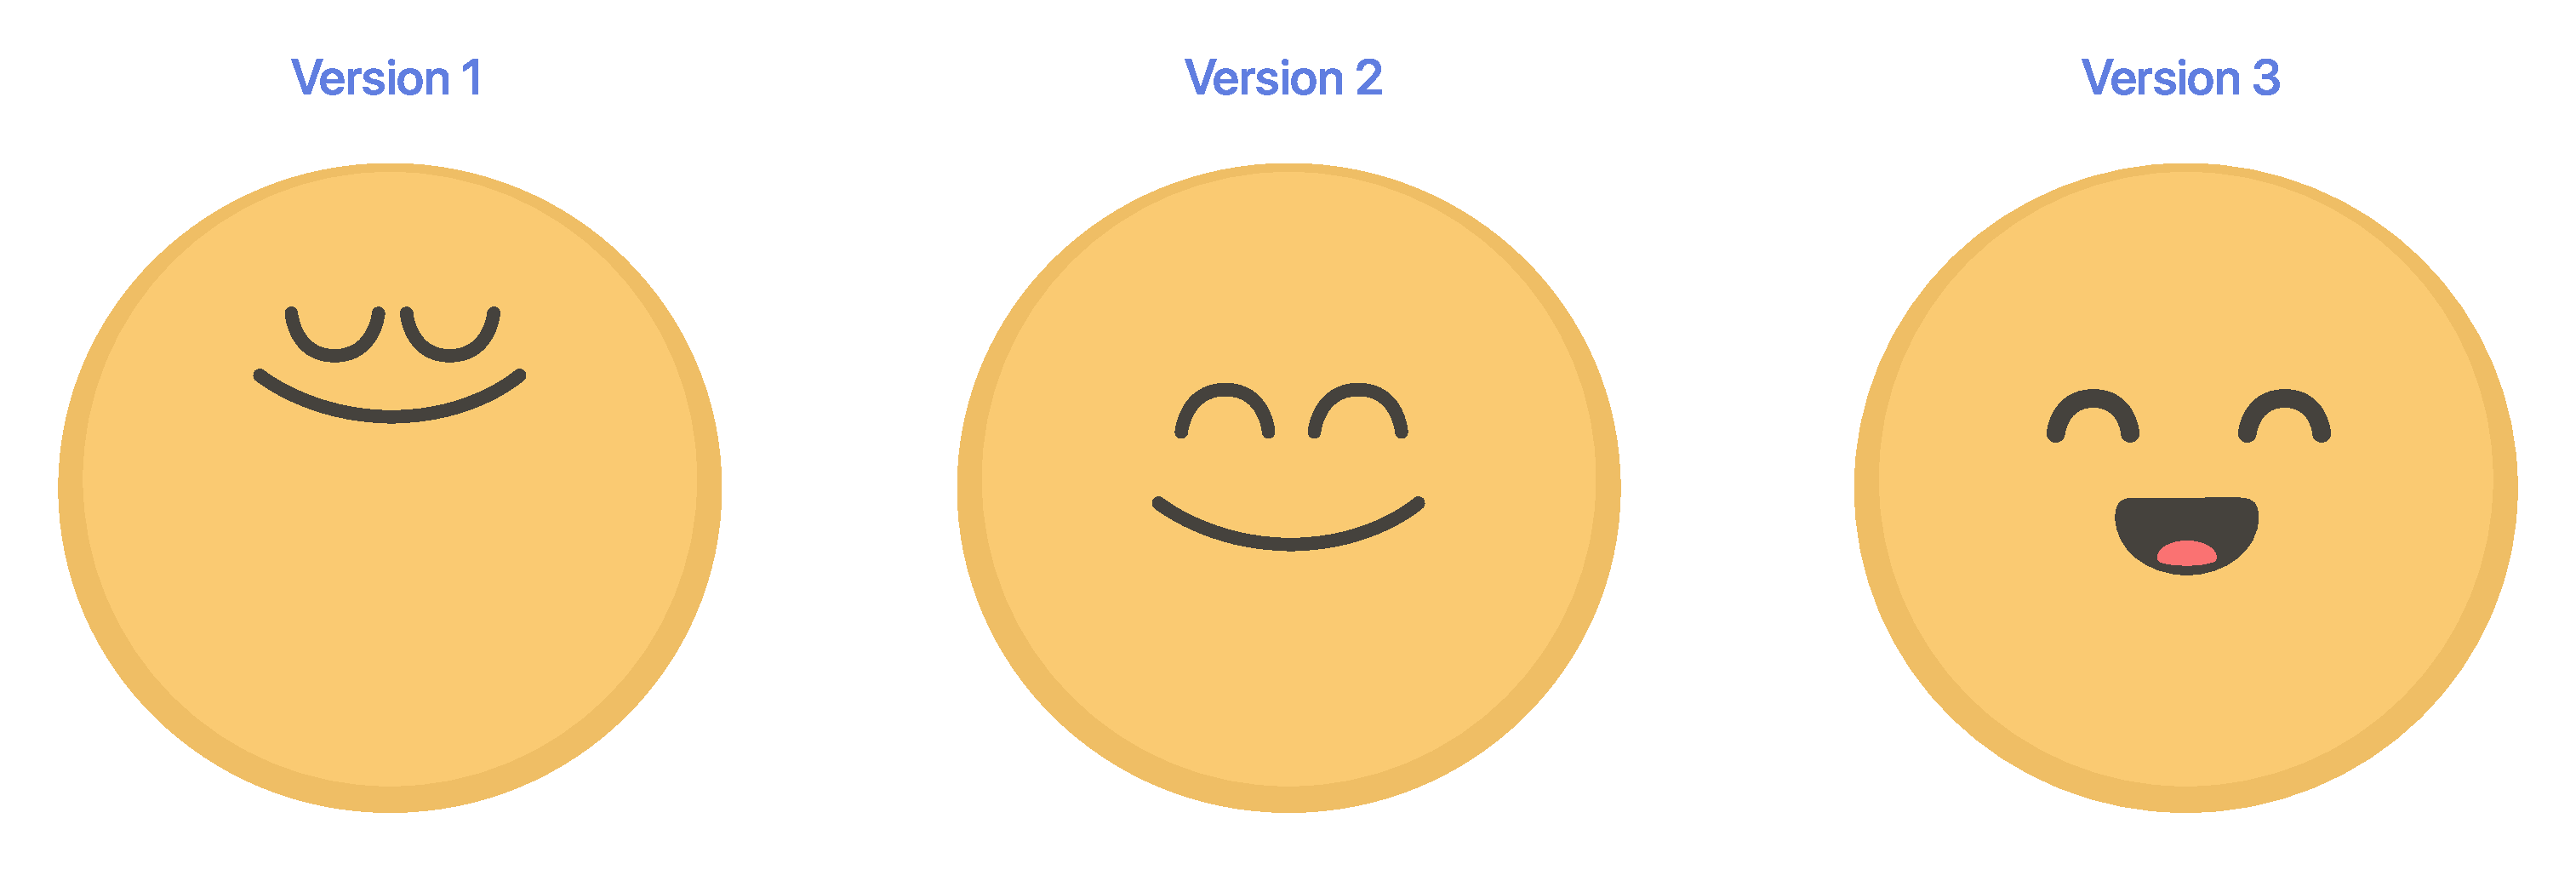
\includegraphics[width=0.7\linewidth]{graphics/smiling-icons}
		\caption{Choice of smiling face icons}
		\label{fig:smiling-icons}
	\end{figure}
	

	\cite{Zorko2017} The impact of the text and background color on the screen reading experience
	
	\clearpage
	\subsection{Experiments}

		\subsubsection{Experiment 1: Short term Memory} \label{sec:memory}
		
		The current memory experiment is based on a commercial "Memory" (TM) game developed in 1966, which has since been widely adopted in digital version on many platforms. 
		In this test participant attempts to match pairs of images which are displayed face down. 
		The constraint is that no more than two images can be turned around at any point in time. Subject begin turning cards at random order until they notice a second card that displays an image that has been turned over before. Once a pair of same images is found they are removed from the game.
		
		The test has been previously used in \cite{McBurney1997} to test memory performance between men and women.
		
		In the current study an adaptation of this game consists of \textit{twenty one pairs} of images that are arranged on a card grid of six by seven cards. Images for the cards in this experiment are taken from the Bank Of Standardized Stimuli (BOSS). BOSS is a set of normative visual stimuli intended for use in cognitive research. library \cite{Brodeur2010}. Images are taken in "png" format with a transparent background and placed on slightly colored card background in the interface. Both living and non-living images are selected. Among them are pictures of fruits and vegetables, technology items, and sport activity items.
		Table (\ref{table:boss-words}) presents the full list of the used BOSS image items in the current study.
		
		\paragraph{Experiment details}
		
		At the beginning of the game the participant is informed that they will see images for ten seconds an need to remember their locations. All images are shown open at the start as a measure to avoid random card selection at the beginning of the game, to allow the participant to identify and get familiar with the image range and selection.
		
		After ten seconds all images turn and the user sees the back-face of the cards in their respective design depending on the theme version.
		
		No practice run is provided in the memory experiment, as it is assumed that the interface and the mechanics of the game are readily familiar to the user \toDo{come back to this assumption in data discovery part}
		
		\paragraph{Activity logging}
		
		\textit{Experiment 1} activity is specified based upon generalized logging of activity in e-learning described in \ref{sec:activitylog}. Activity is logged with two types of actions: events and clicks. They are emitted when each of these conditions are met:
		
		\begin{itemize}
			\item Event: open positions for memorizing
			\item Event: close positions and start game
			\item Event: correct card pair opening
			\item Event: incorrect card pair opening
			\item Click: on card one
			\item Click: on card two
			\item Click: on card when it is inactive (within the timeout delay after click on card two)
			\item Event: memory experiment finished
		\end{itemize}
		
		Card events contain location of the card in the grid, name of image and system context information.
		
		\paragraph{Performance variables:} \label{sec:memory-parameters} Participants \textit{memory performance} is defined by the total number of times any card is turned over. This measure goes in line with the memory test score employed by \cite{McBurney1997}
		
		Additionally, secondary performance measures are defined as follows:
		
		\begin{itemize}
			\item total time taken to solve the test (e1-total-duration-seconds)
			\item amount of cards opened before first incorrect match (e1-pairs-opened)
			\item amount of card opens per minute (e1-opens-per-minute) - as a measure of haste, that could potentially correlate with arousal reports of the users.
			\item amount of clicks on cards made in the timeout phase, when cards are showing two opened cards before they are turned around of marked as solved (e1-inactive-clicks)
			\item amount of pairs opened correctly before first miss (e1-first-miss)
			\item amount of incorrect pair openings (e1-false-guesses = e1-pairs-opened - 21)
		\end{itemize}
	
		These performance variables are calculated and attributed to the participant object for analysis phase.
		
		\subsubsection{Experiment 2: Creative thought} \label{sec:creativity}
		
		A generalized creativity test developed by Mednick \cite{Mednick1962} in 1962 requires the participant to perform creatively. They are "asked to form associative elements into new combinations by providing mediating connective links" \cite[p. 226]{Mednick1962}. This test is called Remote Associates Test or RAT.
		It is developed in such a way that completing it does not require prior knowledge of any particular subject. 
		
		Participants are shown a set of three stimulus words from mutually remote associative clusters. Their task is to provide the mediating link between them. The link must be of an associative manner, rather than one that applies additional logic or inferences. Figure \ref{fig:exampleratset} shows an example of such word-set with a solution.
		
		A possible limitation on the universality of the test is knowledge of language and some cultural influence. Mednick himself states that RAT problems rely on "verbal associative habits could reasonably be assumed to be familiar to almost all individuals that have been brought up in this (USA) culture". The originally presented 30-element list of problems can have a certain degree of dependency on the cultural linguistic habits. For present study additional steps are taken to exclude possible problems due to these effects. 
		
		To minimize the limitation of language knowledge participant is required at the beginning of the study to comply with conditions, which contain (among others) "advanced English knowledge" (Appendix \ref{itm:participation_requirements}). After the tests the participants are asked to state whether or not they are native English speakers and to confirm their English knowledge level.
		
		\begin{figure}[h]
			\centering
			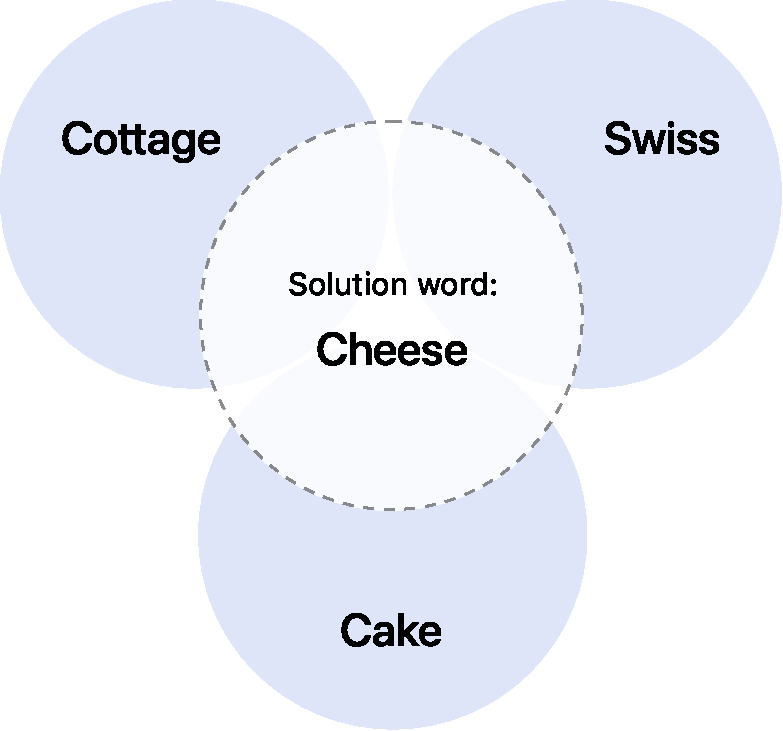
\includegraphics[height=0.3\textheight]{graphics/Example-RAT-Set}
			\caption{Example remote associate word-set 'Cottage, Swiss, Cake'}
			\label{fig:exampleratset}
		\end{figure}

		The current experiment uses a further development of the original Mednick's remote associate test presented by Bowden in a 2003 paper. Bowden et al. \cite{Bowden} have developed 144 sets of remote associate problems with an additional constraint. The solution word has to not only be related to the triad of stimulus words but additionally each of them should form a commonly used compound word or two-word phrase with the solution word. The solution word can build either the first part or the second part of the phrase.
		
		Bowden's word-sets are a subset of all possible remote associate problems and have been alternatively described as "compound word problems".
		
		\toDo{OPTIONAL: longer description of what Bowden proposes with some quotes}
		
 		I select \textbf{twenty} word-sets of a set of 144 compound remote associate sets that are proposed by \cite{Bowden}. Some of the easier (highest solving percentage rate among the 30-second threshold test participants, as provided by Bowden) word-sets are selected for present experiment. Additional filtering is applied to avoid colloquialisms and words that can be regarded as a local expression. As a result, the twenty word-sets should be challenging although solvable to a wide array of people from different backgrounds. Having very limited time and amount of words due to the experiment design, I attempt to maximize solution rates. Once the time to solve a problem runs out the problem is marked as unsolved for this participant session. Without a high degree of solved problems it gets more difficult to compare results.
		One of the indicators for performance is the time taken to solve a problem. (\ref{sec:creativity-parameters}).
 		
 		Table \ref{table:selected-remote-associates} presents the full list of the used RAT items in the current study. 
		
		\paragraph{Experiment details}
		
		Before the experiment begins, the participant is informed about the rules and what is expected from them with an introductory text:
		
		\begin{displayquote}
			"You will see three stimulus words. Attempt to generate a fourth word that is related to each stimulus word. When combined with each of the stimulus words will build a word pair that is a common compound word or phrase. The goal is to find a solution as fast a possible
			
			After 30 seconds you will see 2 words appearing as hints on the screen, only one solution is correct.
			The first 3 are practice sets and will allow you to train. During practice we will give you a hint after 10 seconds"
		\end{displayquote}
	
		The participant is shown three practice tasks which allow them to get used to the interface and the dynamics of the task. As most of the participants are remote and unsupervised it is important to give an intuitive set of instructions and avoid any confusion or variation due to unclear interface or task.
		
		\begin{figure}[h]
			\centering
			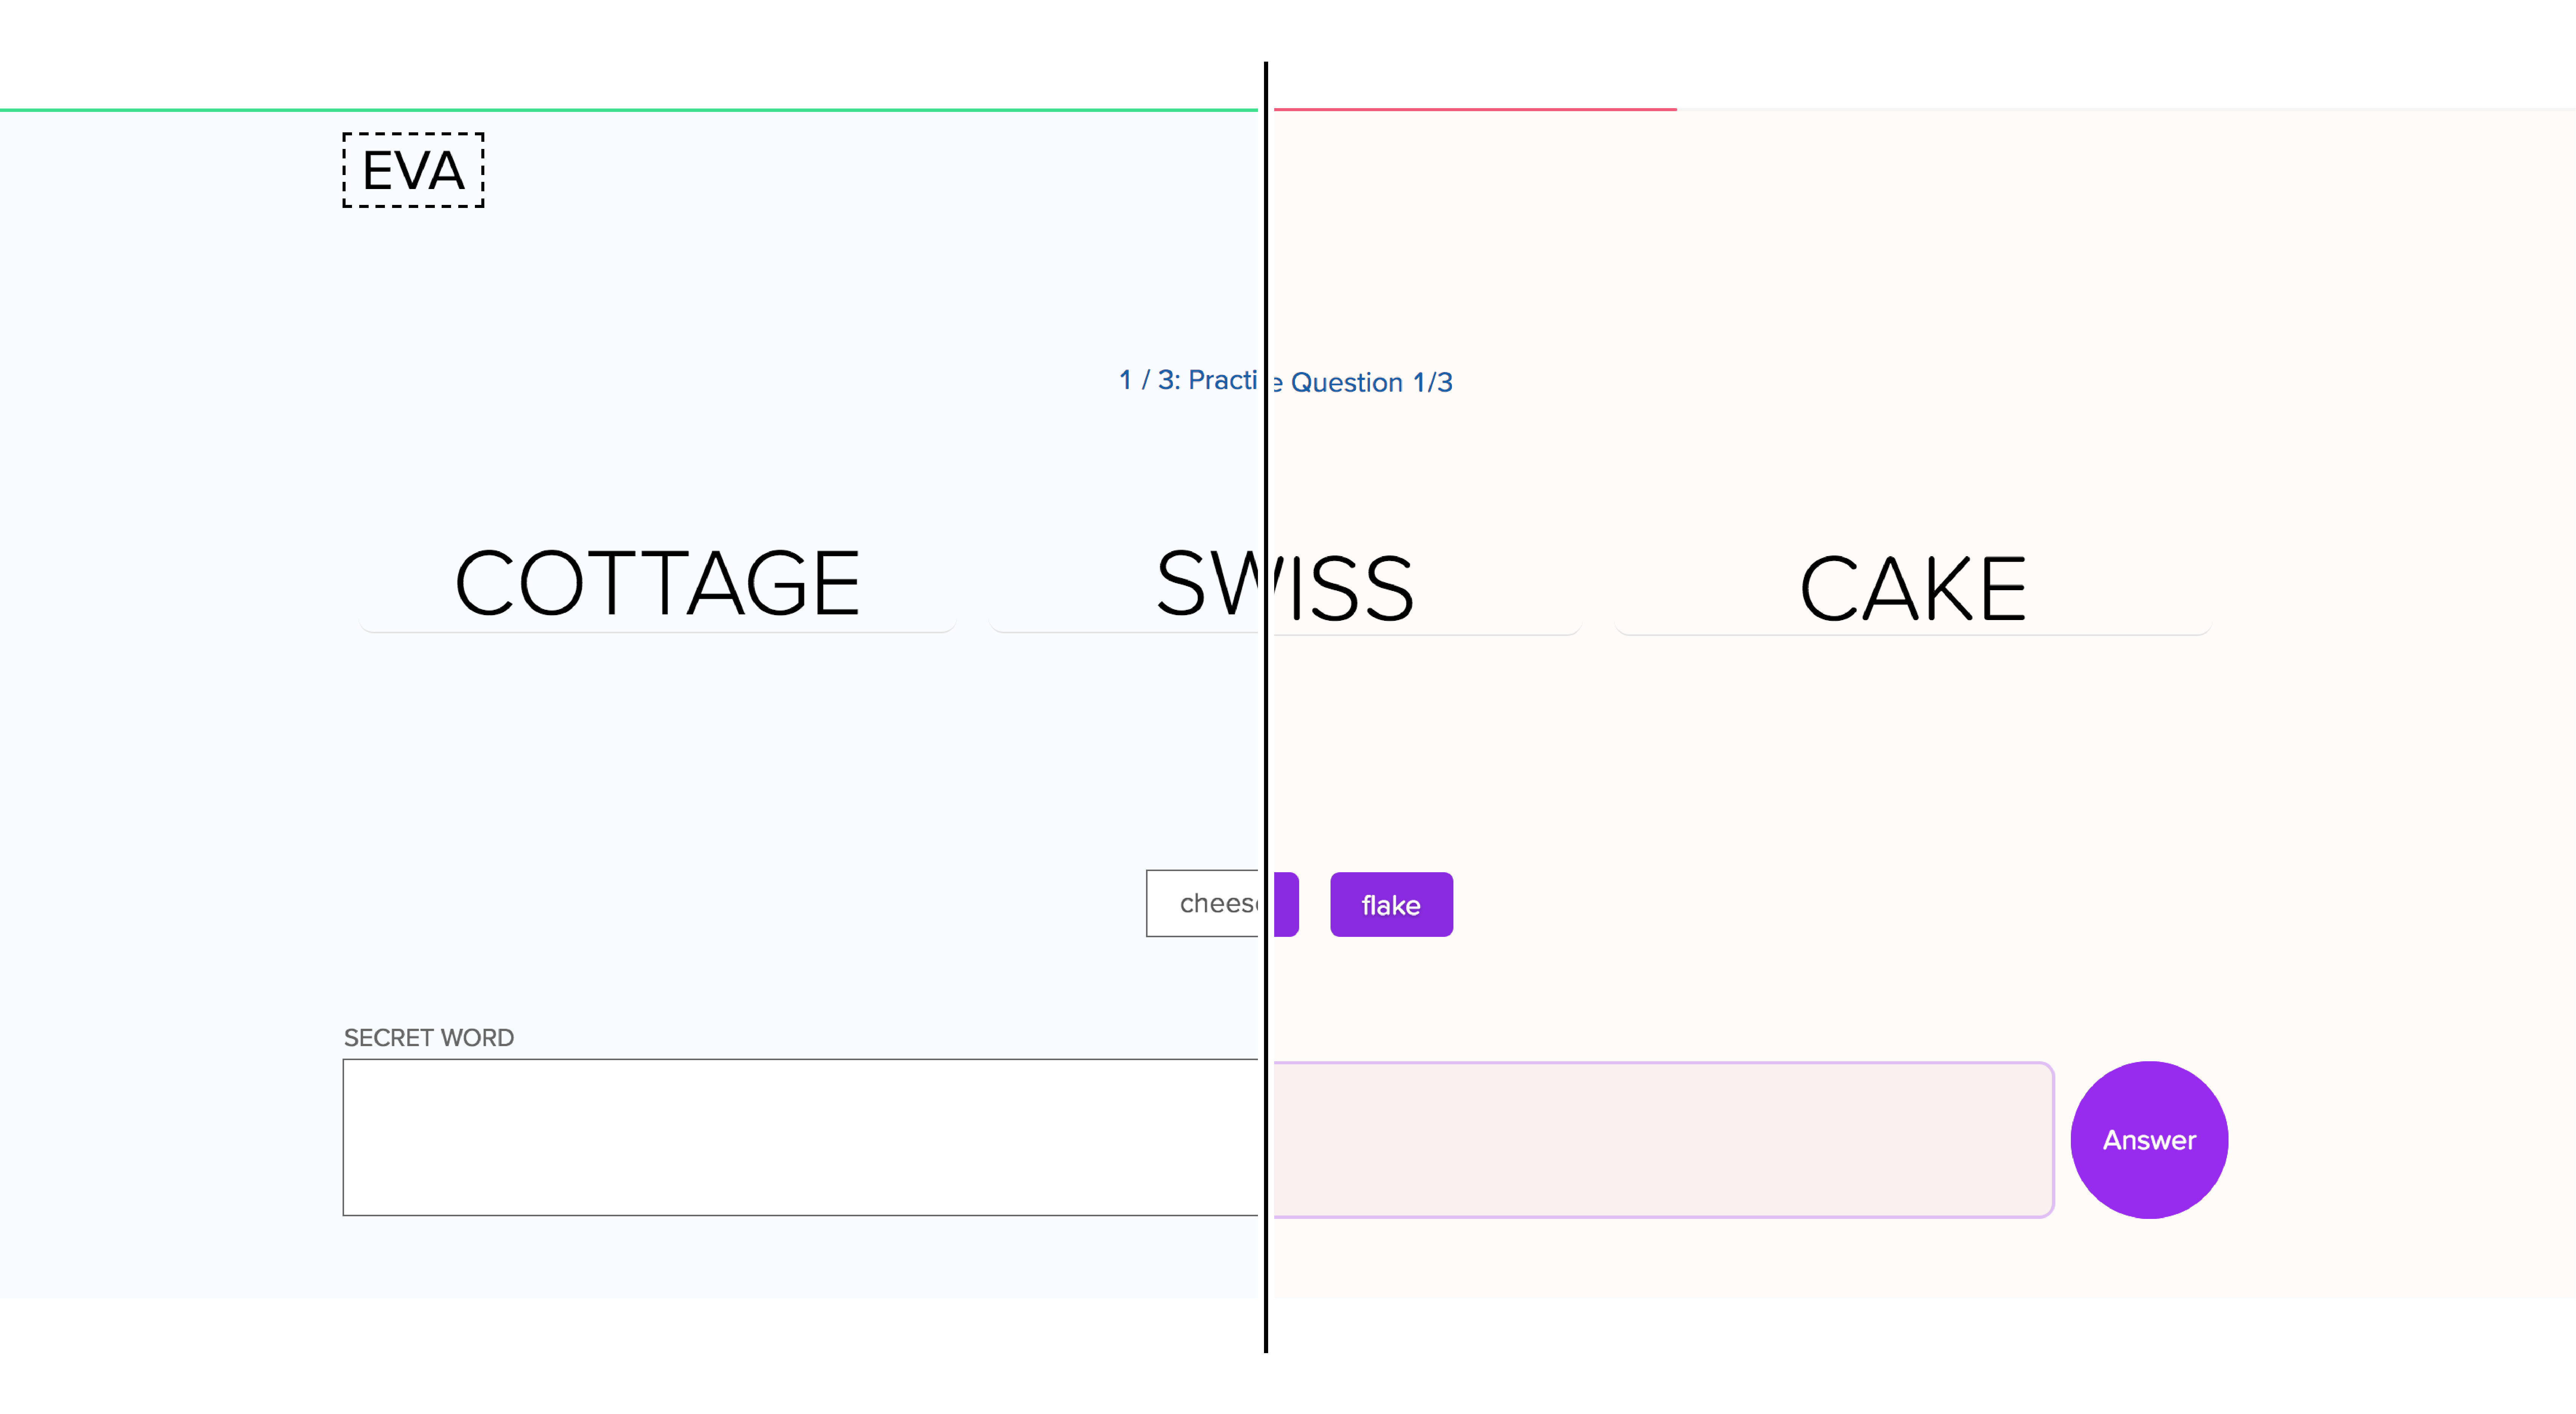
\includegraphics[width=0.7\linewidth]{graphics/creativity-versions}
			\caption{Example screen showing both versions of interface during creativity experiment}
			\label{fig:creativity-versions}
		\end{figure}
	
		After 3 practice tasks, participant clicks on "Start Experiment" before solving 20 items defined in the set. An example preview of both interface screens with the three stimulus words and an input for the answer is displayed in figure \ref{fig:creativity-versions} 
		
		Upon appearance of each word-set a timer starts tracking the time to enter a word.
		Stimulus words appear with a 200ms delay from timer start and 50ms delay between each word appearing. The appearance animation takes 300ms. All items are completely visible at 600ms mark, with the first word in the left-to-right direction completely visible and static at 500ms after timer start. 500ms can be discounted from the time it takes to solve a problem (Effectively participants have 29.5 seconds to solve a problem).
		
		\subparagraph{Appearance of Hints}
		
		Each word-set has a 30 second limit to solve a problem. After time is expired a block with 2 hint words (illustrated in figure \ref{fig:hint-buttons}) appear. One of them is the correct solution to the problem, another is a false answer. It is semantically clear which solution is correct, upon reading it the participant is expected to experience the "aha!" effect mentioned in \cite[p.634]{Bowden} with a reference to previous research. Choosing the wrong answer once the time expires can be a hint that the participant is not paying attention. After hints appear, the problem is no longer counted as solved by the participant.
		
		\textit{Hints appearance can be delayed.} Due to a person requiring time to type the answer on a keyboard it is assumed the answer is known once the first letter of the word is written in the field. There is a 3000ms grace delay to type each additional character. Grace delay accounts for typing speed and is deemed as sufficient for most persons. Erasing a character is considered as typing (and resets the counter) unless the first letter of the input is erased. Once the delay is passed or the first letter erased the hints appear and the problem is marked as unsolved. Time of the first letter being typed is considered an objective point of time that a participant figures out the answer to the problem. The time of first letter is always within thirty seconds of appearance of the word-set.
		
		\begin{figure}
			\centering
			
\includegraphics[width=0.3\linewidth]{graphics/Hint-buttons}
			\caption{Hints after time allowed for solving a problem is elapsed, example words are provided from the practice test}
			\label{fig:hint-buttons}
		\end{figure}
		
		Once all items are solved they are directed to the next page of the interface.
				
		\paragraph{Activity logging} \textit{Experiment 2} activity is specified based upon generalized logging of activity in e-learning described in \ref{sec:activitylog}
		
		A generic action emitter triggers an action when either of the following happens:
		
		\begin{itemize}
			\item Click on button to start practice
			\item Click on button to start live experiment
			\item Event when word set appears on screen
			\item Event when word set is guessed correctly
			\item Event when word set is guessed incorrectly
			\item Event when word set has expired (hint words appear)
		\end{itemize}
	
		Each event object contains system status information and context information about current words visible.

		\paragraph{Performance variables} \label{sec:creativity-parameters}
		
		A range of metrics are calculated and attributed to each participant for analysis:
		
		\begin{enumerate}
			\item Aggregated solving speed: seconds taken to solve a problem on average (e2-avg-duration-per-word)
			\item Non-aggregated solving speed: seconds taken to solve each problem (e2-word-*)
			\item Idea generation rate: how many attempts (including false ones) are taken within the time limit on average (e2-idea-rate)
			\item Success rate: Number of problems solved successfully (e2-correct-guesses)
			\item Frustration/Negative-attention: Amount of false choices after \textit{Hint Word} suggestion appears as ratio to Hint Word suggestion answers. (e2-neg-attention-ratio)
			\item Total points (time left for all words, e2-total-points)
		\end{enumerate}
	
		The e2 performance variables are calculated and attributed to the participant object to be used during the analysis phase.
		
%		\toDo{elaborate about the measures and reasoning behind them}

	\subsection{Means of emotional self-evaluation} \label{sec:selfeval}
%	

% \todo[inline, size=\tiny]{'Valence and Arousal evaluation techniques'}


	\toDo{Describe Valence and Arousal evaluation methods}  \cite{Harley2016}
	
	SAM , AS, Affect Grid \cite{Russell1989} (the same guy who created the circumplex model 9 years prior), 
	AffectButton \cite{Broekens}
	
	A positive Affect Scale (PAS) from the Positive and Negative Affect Schedule (PANAS; \cite{Watson1988}).
	
	Due to effort constraints of the participants it is important to achieve a intuitive, quick, yet accurate reading of their emotions. In the context of this study self-evaluation is a means to validate results, of Hypothesis 1. I rely on the SAM (Self-Assessment Manikin) method \cite{Bradley1994} to quickly allow users to assess their emotions on a dual 9 point scale. Figure \ref{fig:sam} illustrates the structure of the self-assessment screen.
	
\begin{figure}[h]
	\centering
	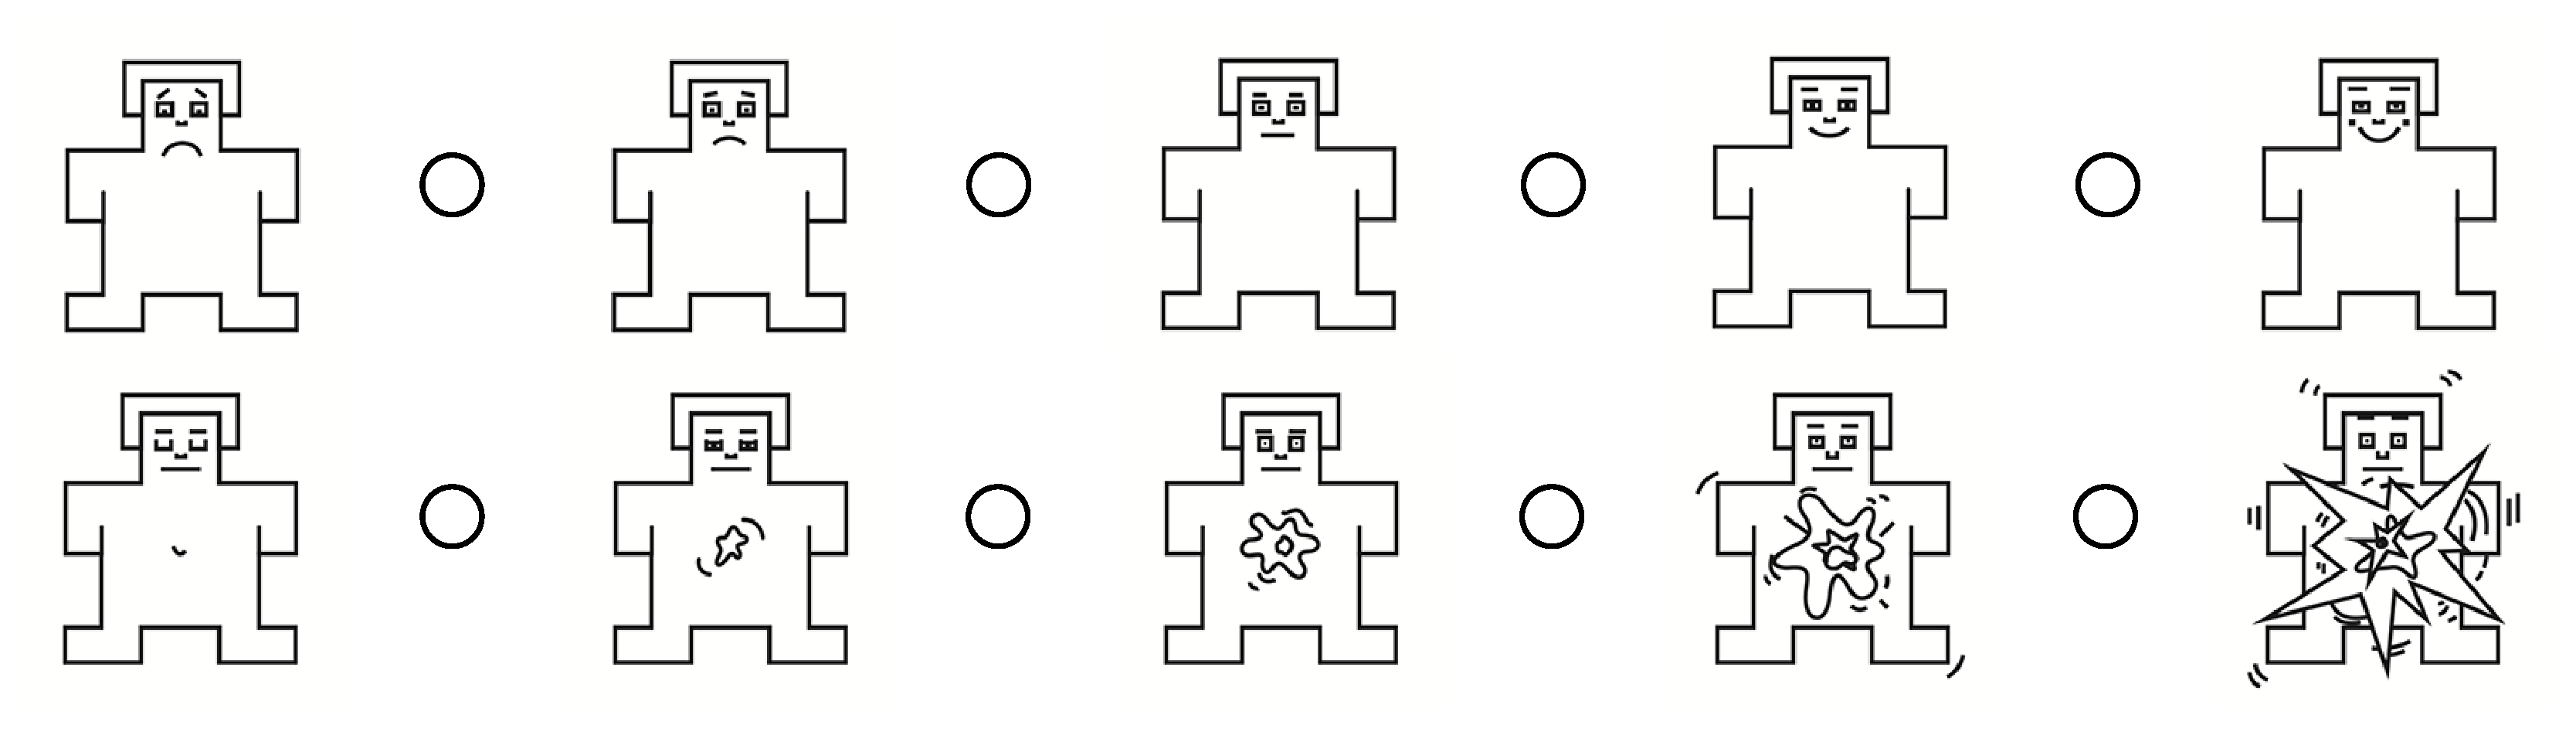
\includegraphics[width=0.9\linewidth]{graphics/SAM}
	\caption{Self-Assessment Manikin. Input for valence and arousal values on nine-point scale}
	\label{fig:sam}
\end{figure}
	
	\subsection{Demographic data and supplemental information} \label{sec:demographics}
	
	As final step of the study each participant fills out a demographics questionnaire to add context data and help with analysis. There are 4 questions:
	
	\begin{enumerate}
		\item Gender \\ \ [Male / Female]
		\item Age \\ \ [18-24 / 25-29 / 30-34 / 35 - 44 / 45 + ]
		\item Is English your native language? \\ \ [yes / no]
		\item What is your level of English knowledge? \\ \
			[Beginner  / Intermediate / Advanced / Fluent]
		\item Occupation: \\ \ [High school student / Undergraduate Student / Graduate Student / Doctorate / Professional or Working]
		\item Email (optional)
	\end{enumerate}

	Gender (Question 1) allows to uncover difference in performance or response due to gender. Possible disparities are expected to be observed as described in \ref{sec:preconditioning}

	The age groups (Question 2) are taken in accordance with suggestions provided by the Standard International Age Classifications \cite{UN1982} with slight modifications to exclude ages below 18.
	
	%Ages above 44 could potentially skew results due to factors not considered by present study. Primary focus audience lies between ages of 18 and 34.
	
	Native speakers (Question 3) might potentially score higher on the creativity task due to cultural influence of using colloquial expressions. This assumption is challenged during data analysis in section \ref{sec:data-validity}
	
	(Question 4) is used to validate the requirement of at least an "advanced" proficiency in English. Participant choosing anything lower could suggest either invalid data or problems with the creativity task due to language issues. In this case participant is considered for removal. \todo{evaluate this claim}
	
	Occupation is inquired for additional context into the participant.
	
	Final "email" field allows the user to enter their email address for participation in the raffle and complies with the motivational promise at the beginning of the experiment.

	\subsection{E-learning activity logging} \label{sec:activitylog}
	%To assess performance of subjects several measurements are taken during the test, these differentiate between the 2 experiments.
	
	Each participant is defined as a \textit{user}. Each user is assigned a session for each new started experiment. 
	
	To assess the performance of participants continuous measurements are taken during a session of the experiment. A general approach is an event-based system where each \textbf{action} from the \textit{user} or the \textit{system} is emitted to the database. A differentiation is established between a "click" action that is initiated by the user and an "event" action that is initiated by the system environment.
	
	For correct attribution at the moment when action is emitted it contains: 
	\begin{itemize}
		\item userID, sessionID, timestamp (unique key)
		\item name of active screen
		\item type of action (\textit{event} or \textit{click})
		\item context information such as global system state and dependent values of current active screen
	\end{itemize}

	Finally, for system actions (events) \textbf{name of event} is provided. For user actions (clicks) a target of the click is provided.
	
	%A session is defined on the scope of single e-learning module and contains user metadata as well as emotional state of the learner.

	

		
		\paragraph{Technical implementation}
		
		Upon requesting the page a user-token is generated and assigned to each participant. This token is saved as a cookie for future reference and visitor matching. Only one successful experiment is allowed per participant due to 
		Each experiment further contains a session object with its attributes. 
		
		"[location]\_[action]\_[result]"
		
		\toDo{[TODO:] describe how tracking is implemented, storage and analysis for current study}
		
		Action tracking is managed by a dedicated module that communicates with the database storage API. Each event sent to the Database is complemented with a timestamp and user data. An action object with usual fields is described in listing \ref{lst:db_object}


	\begin{listing}[h]
		\begin{minted}{json}
			{
			"first": "second1"
			}
		\end{minted}
		\caption{Database Object Fields}
		\label{lst:db_object}
	\end{listing}

\toDo{specify object}

		
		\paragraph{xAPI adaptation} - 
		
		\toDo{[Optional:] explore adaptability and possible constraints}

\section{Study implementation}

\paragraph{Participant sourcing} 
This study includes participants attained through multiple sources:
\begin{itemize}
	\item{Local university:} On-site supervised experiments were conducted on a limited scale to facilitate a clean sample of participants and uncover problems during the study
	
	\item{Local workplace:} On-site semi-supervised experiments are conducted on a limited scale in Berlin area in Germany to facilitate a more diverse sample while keeping controlled environment conditions, similar to university experiments.
	
	\item{Social media:} Remote participants are invited to participate in unsupervised experiments on their own. Channels such as social media, interest groups and university mailing lists are used.
	
	\item{Mechanical turk:} MTurk is one of popuar web services to source participants. Previous research has shown that it can be considered a reliable platform for conducting objective studies. MTurk participants receive monetary compensation for participation \cite{Buhrmester2011a}. Mturk participants are excluded from motivation with a chance on winning a voucher prize (they do not see the field and information box about it), instead regular participant reward through MTurk is used.
	
\end{itemize}

Local and social media experiments provided additional motivation of participation with the promise of a chance to win a 20 Euro Amazon-voucher.

\subsection{Technical implementation} \label{sec:study_technical_implementation}
At the base of current implementation is the requirement to run the study in a browser on a personal computer. 

As the study is done in the field and participants are not supervised I introduce additional checks to ensure that only one session can be completed per one participant. Upon visiting the first page the user retains several cookies that identify them later in the data and during subsequent visits: \textit{userID, sessionID}. UserID is persisted across visits, while sessionID is generated each time the page is loaded and consists of `userID+timestamp`. Once the participant finishes the experiment the session is marked as finished and a cookie is placed on the participant machine.

\paragraph{Theme propagation} React.js is selected as a library of choice due to it's favorable characteristics to creating an environment that supports 2 themes and global settings in a scalable way. React's unidirectional data flow allows clear behavior path between application data and visual representation. In particular, it becomes possible to adjust the theme of the interface and propagate in-place an alternative style and visual rules throughout the application without losing current state. Additional benefits of this approach are discussed in section \ref{sec:further-research} in the context of an emotionally aware interface.

\begin{figure}
	\centering
	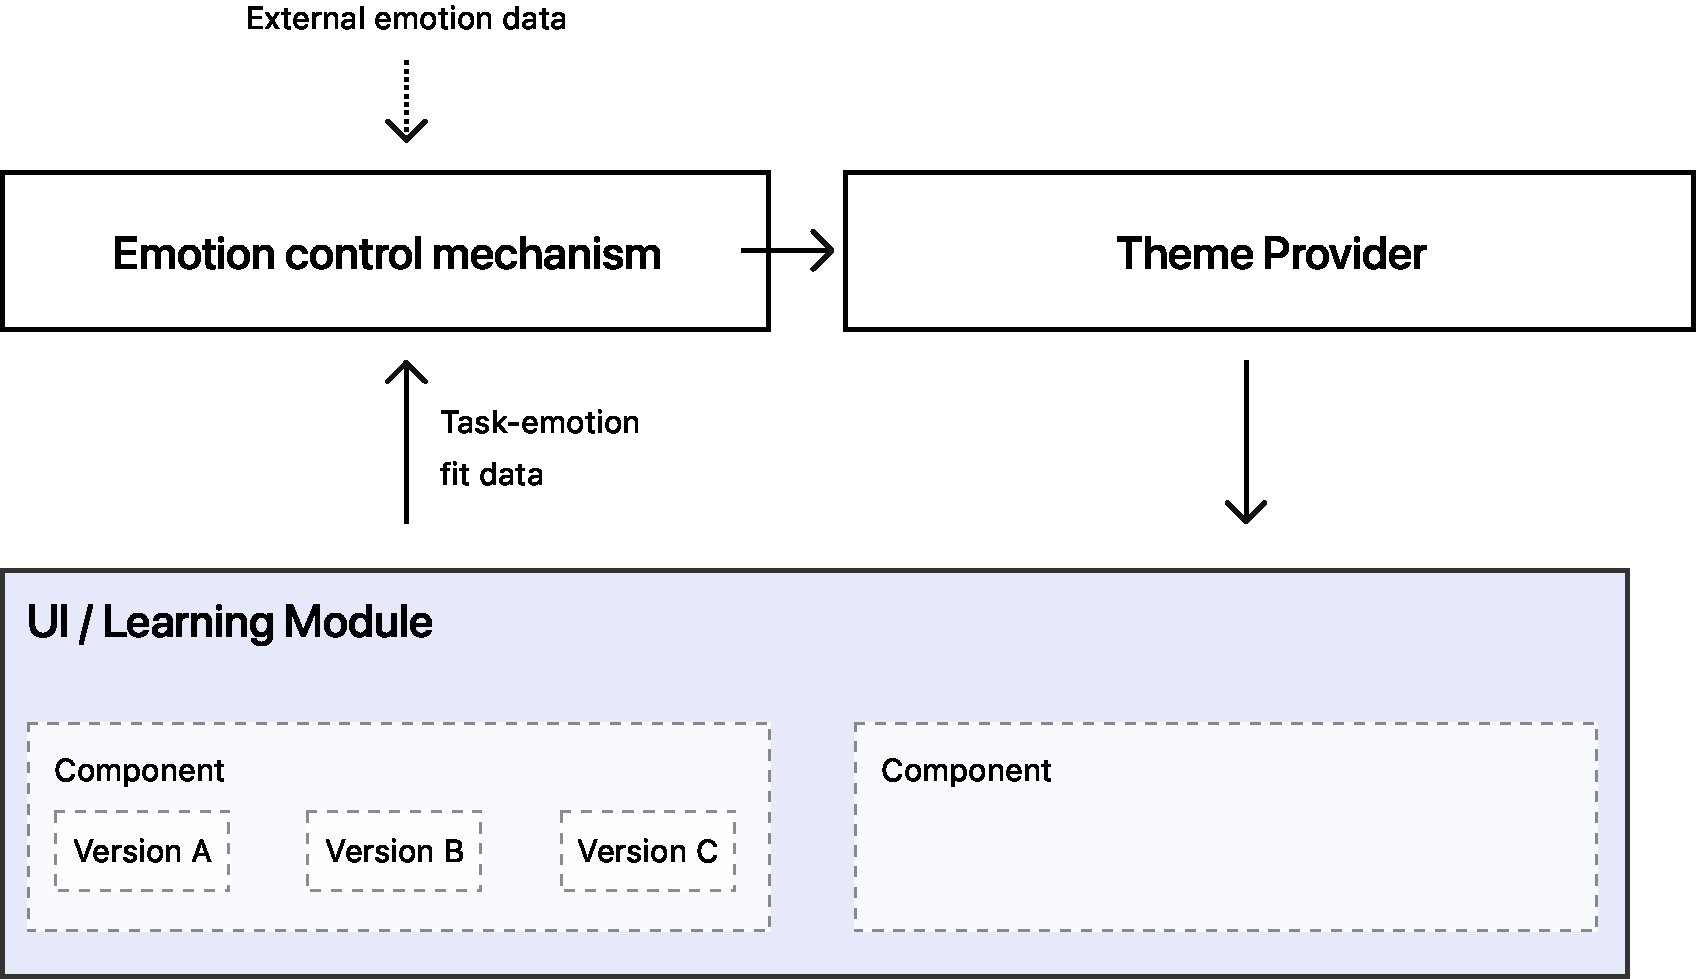
\includegraphics[width=1\linewidth]{graphics/App-Architecture}
	\caption{Component based architecture with emotion control mechanism}
	\label{fig:app-architecture}
\end{figure}

Current implementation contains a minimal proof-of-concept of a way to enable e-learning interfaces to be complemented with emotional data. 

As described in section \ref{sec:research}, research made by \cite{Haaranen2015} puts forth the need to acknowledge current learning context, when deciding on an appropriate emotional-interface response. 
Some emotional-design features may fit best an e-learning module than others.
For example creative tasks might be supported with a warm-colored interface and providing strong degree of control to the user to play around with elements on the screen. 
And analytical tasks might require more concentrated thinking, they might profit from absence of additional distractions, such as images or not directly relevant text. "Seductive details" might cause the learner to concentrate on the wrong content, as proposed by the distraction hypothesis (Harp \& Mayer, 1998) and revisited in \cite{Chang2014}.
Furthermore a distinction can be drawn by learning topic - serious topics can require stricter presentation rules, than entertaining e-learning content.

With the architecture illustrated in Figure \ref{fig:app-architecture}) it is possible to develop an interface that responds to emotional and task contexts with an appropriate interface. A split between presentation layer - UI/Learning Modules, and an "Emotion control mechanism" as well as a "Theme Provider" layer orchestrating UI-level decisions on a global level allows to adjust visual presentation on the fly and from screen to screen.

Learning Modules submit task-emotion fit data to the emotion control layer when each module loads. The emotion control layer then decides on the correct presentation fit which it then passes to the Theme Provider. Additional data about the users emotions can be submitted via self-reporting or through ambient and body-sensors. For the purpose of the study current implementation does not take into account user's self reported emotional affect to adjust the theme. This implementation assigns a theme version at load time and keeps it constant over the course of the experiment.

\section{Results}

	\subsection{Collected data}
	
	Overall one hundred and five (\textbf{105}) respondents have completed the experiment. Among these 58 (55.2\%) people have been acquired through Amazon Mechanical Turk service, while 47 (44,8\%) have been recruited through social platforms, and local/university. Incentivisation is provided through direct payment for completion or a raffle after the study, respectively.
	
	\paragraph{Population distribution}
	
	In sum forty one (39\%) female participants and sixty four (61\%) male participants finished an experiment session (Table \ref{tbl:gender-distribution}).
	 
	Across five age groups, 11 (10.5\%) participants selected 18 - 24, 34 (32.4\%) are between 25 - 29  years old, 28 (26.7\%) between 30 - 34, 20 (19\%) between 35 - 44, and 12 (11.4\%) are 45 years old or older.
	
	Most popular occupation group is a "Professional" with 65 (61.9 \%) participants reporting it, 17 (16.2\%) in undergraduate studies, 16 (15.2\%) in graduate degree program, 2 (1.9\%) doing a doctorate, as well as 5 (4.8\%) respondents in high school at the moment of participation.
	
\begin{table}[h!]
	\centering
	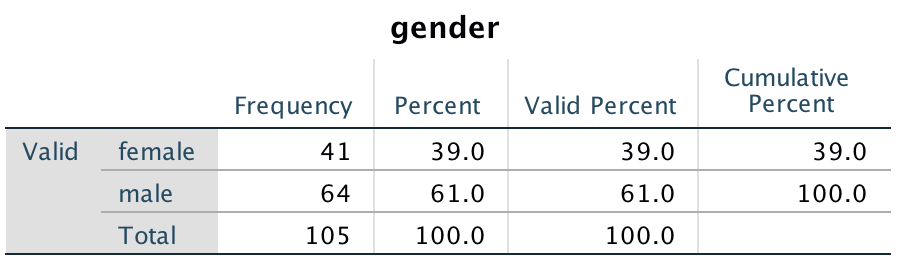
\includegraphics[width=0.7\linewidth]{graphics/Gender-distribution}
	\caption{Distribution of participants by gender}
	\label{tbl:gender-distribution}
\end{table}
	
	\paragraph{Affect levels} Participants rated their mood a total of 3 times, with the first rating making a baseline before testing begins. Valence and arousal values are rated on a 9 point scale with "1" being the lowest rating and "9" - the highest. Table \ref{tbl:distributionOfAffect} shows the affect ratings per preconditioning group. Post Task values include both theme versions in this table. On average participants began with a slightly positive valence (mean 6.08, SE 1.36) and a slightly low level of arousal (mean 3.78, SE 1.8).
	
	\begin{table}[h!]
	\begin{center}
				
		\begin{tabular}{|c|c|c|c|c|}
			\hline 
			& \multicolumn{3}{c|}{Rating} &  \\ 
			\hline 
			Preconditioning & Initial (1) & Pre Task (2) & Post Task (3) & Observations \\ 
			\hline 
			& \multicolumn{3}{|c|}{Arousal} &  \\ 
			\hline 
			Angry (0) & 3.83 (1.83) & 5.09 (2.15) & 5.04 (1.9) & 23 \\ 
			\hline 
			Happy (1) & 3.72 (1.99) & 4.84 (2.08) & 4.75 (1.95) & 32 \\ 
			\hline 
			Sad (2) & 3.82 (2.08) & 3.95 (1.81) & 4.45 (2.11) & 22 \\ 
			\hline 
			Calm (3) & 4.00 (1.68) & 3.46 (1.53) & 4.54 (1.97) & 28 \\ 
			\hline 
			& \multicolumn{3}{|c|}{Valence} &  \\ 
			\hline 
			Angry (0) & 6.17 (1.19) & 2.39 (1.41) & 5.57 (2.00) & 23 \\ 
			\hline 
			Happy (1) & 5.81 (1.42) & 6.12 (1.39) & 5.00 (2.02) & 32 \\ 
			\hline 
			Sad (2) & 6.41 (1.44) & 4.18 (1.50) & 5.59 (1.56) & 22 \\ 
			\hline 
			Calm (3) & 6.29 (1.36) & 6.07 (1.41) & 5.75 (2.08) & 28 \\ 
			\hline 
		\end{tabular}
	\end{center}
	\caption{Mean (and Standard Deviation) for each preconditioning}
	\label{tbl:distributionOfAffect}
	\end{table}

	\paragraph{Age}
	
	Each Participant stated their age group. Across all participants the distribution is as follows: Group 18 - 24: \textbf{11};
	Group 25 - 29: \textbf{34}; Group 30 - 34: \textbf{28}; Group 35 - 44: \textbf{20}; and finally group 45 and above with \textbf{12} participants.	

	\paragraph{Distribution by english knowledge} 
	
	
	
	\subsection{Data Preparation}
	
	\subsubsection{Unique participants check} First, a test is made whether all completed experiment sessions are done by a unique user to avoid interference, due to exposure to study in a previous run. Multiple participation are to be excluded, with only the first session being valid under this study design. An SQL query (\ref{itm:sql_check_single_session_per_user}) confirmed, that no participant finished the study multiple times.
	
	\begin{table}
		\begin{center}
			\begin{tabular}{|c|c|c|c|}
				\hline
				\multicolumn{4}{|c|}{Participant Attributes} \\ 
				\hline 
				source & preconditioning & theme-version & age \\ 
				\hline 
				gender & education & englishlevel & native \\ 
				\hline 
				arousal-preprecond & arousal-pre & arousal-post & quadrant-pre \\ 
				\hline 
				valence-preprecond & valence-pre & valence-post & \\ 
				\hline 
				e1 total duration (sec) & e1 pairs opened & e1 false guesses & e1 opens/minute \\ 
				\hline 
				e1 inactive clicks & e1 first miss & e1-avg-click-delay &  \\ 
				\hline 
				e2 avg time/word & e2 time left [word.*]  & e2 idea rate & e2 correct guesses \\
				\hline
				e2 sum bad hint-clicks & e2 neg attention ratio & & \\
				\hline
			\end{tabular} 
		\end{center}
		\caption{Participant attributes}
		\label{fig:participant_attributes}
	\end{table}

	\subsubsection{Defining Attributes} Initial events-based data is transformed into metrics for each participant as displayed in table (\ref{fig:participant_attributes}). Prefix "E1" prefix represents Experiment1 (Memory test), and Prefix "E2" represents Experiment2 (Creativity test). \textit{Arousal-preprecond} and \textit{valence-preprecond} are the values measured initially at the start of the experiment before any intervention. Variables \textit{arousal-pre} and \textit{valence-pre} represent the measurement after preconditioning step. Finally, \textit{arousal-post} and \textit{valence-post} are the values that are reported by participants after finishing both experiment tasks.

	\paragraph{Emotion quadrants}
	
	Valence and arousal values are transformed into quadrants with the split in both axes at the value 5:
	\begin{enumerate*}
		\item Q1 = (arousal >= 5 \& valence  < 5)
		\item Q2 = (arousal >= 5 \& valence  >= 5)
		\item Q3 = (arousal < 5 \& valence  < 5)
		\item Q4 = (arousal < 5 \& valence  >= 5)
	\end{enumerate*}. Resulting variables are \textit{quadrant-initial}, \textit{quadrant-pre}, \textit{quadrant-post}.
	
	\paragraph{E1 metrics} \label{sec:e1metrics}
	
	E1 performance variables are described in section \ref{sec:memory-parameters}. Following consideration is dedicated to choosing the right objective performance metric and discussion on applicability of others based on received data.
	
	Due to differences in the theme versions the delay for after opening a pair before then next card can be clicked is different. 750ms compared to 1200ms. This delay can cause people to wait longer than they want between opening pairs.
	
	A similar delay of 450ms can be caused between opening first and second card due to animation in theme version "1" which has a delay of 600ms with the image clearly seen after 450ms. Metrics that are dependent on time (e1-total-duration-seconds and e1-opens-per-minute) are not readily comparable for participants across two different theme versions. To test this I compare the real click delays based on the \textit{e1-avg-click-delay} variable.

	\subparagraph{Click delay between card1 and card2 clicks across theme versions} Dependent variable "e1-avg-click-delay" is analyzed through independent samples t-test on the factor variable "theme-version", to see if there are differences in click delay between theme versions.
	
	As assessed by an inspection of the box-plot some outliers are present in the data. As I am taking the average click delay of participants, their respective value can be skewed by the underlying data. The original event data shows some participants taking a disproportionately longer breaks between clicks. Either they were distracted by something or they took their time to select the second card. Some participants taking longer belong to the age group "45plus". In this case the delay could be explained by a slower mouse movement to target. At the same time some participants (those who have a maximal click delay of more than 10 seconds) were apparently distracted, with one participant taking more than 744 seconds to click on card2. As a result I decided that these outliers are not representative of the general click-rate. Six outliers are removed for this statistical test.
	
	Average click delays are normally distributed for each level of the theme version, as assessed by Shapiro-Wilk's test (p > .05, actual values for theme0 with p = 0.307, theme1 with p = 0.374). Among 47 participants with theme0 and 52 with theme1, those getting theme0 have had a shorter delay between clicks on the first and second cards (M = 1 093ms, SD = 227ms), while those getting theme version 1 spent longer to click on the second card (M = 1 537ms, SD = 332ms). The click delay for theme0 is 443ms, 95\% CI [556 to 330] shorter than for theme1. The results are statistically significant (based on Welch t-test) on a p < 0.001 confidence level ( t(90601) = -7811 ).
	
	According to this analysis, the delay difference of 443ms, which is highly similar to the 450ms predicted due to animation length and character (accelerated rotation) makes time based metrics not applicable for comparison between theme0 and theme1 in their original state.
	
	Based on these findings the most objective E1 performance metric appears to be \textit{e1-pairs-opened}.
	\textit{e1-first-miss} might further give insight on the single instance of memory performance at the beginning of the game after 10 seconds of memorization.
	
	\paragraph{E2 metrics}
	
	E2 performance variables are described in section \ref{sec:creativity-parameters}. Following consideration is dedicated to choosing the right objective performance metric.
	
	Event based data structure allows to extract a series of E2 metrics that describe a participants behavior:
	\begin{itemize*}
		\item e2 avg-time 
		\item e2 time left [word.*]  
		\item e2 idea rate 
		\item e2 correct guesses
		\item e2 sum bad hint-clicks 
		\item e2 neg attention ratio
		\item e2 total points
	\end{itemize*}
	
	Unlike the first experiment, creativity experiment has no timing differences across theme versions and can therefore include time-based metrics as a measure of performance for comparison across versions.
	
	The primary measure of participant's \textit{creativity performance} can be most objectively defined by the sum of time left to solve a word at the moment of solving it (described by \textit{e2-total-points}). For example, solving a word-set within 10 seconds will result in a 20 point gain (30 seconds available - 10 seconds used). The sum of all words results in a continuous variable with the minimum of 0 (word is not solved) and a maximum of 30 (word is solved instantly) points per word. The measure has an advantage over a simpler \textit{e2-correct-guesses} due to its granularity. Participants who guessed the word quicker would be ranked higher than the ones who took longer, even when the amount of words guessed is equal. Additionally, due to the way the time left is calculated, typing speed is irrelevant and does not influence the points total.
	
	Consequently, E2 performance measure for current analysis is \textit{e2-total-points}.
%		\textit{e1-first-miss} might further give insight on the single instance of memory performance at the beginning of the game after 10 seconds of memorization.
	
	
	
	\subsection{Validation of assumptions} \label{sec:data-validity}
		
		\subsubsection{Female participant reaction to "happy" preconditioning}
		
		Laboratory tests with female participants provided feedback, that "happy" preconditioning which contains some sexually suggestive images or a female body, does not yield a positive effect on valence. Following analysis provides a check whether female reactions to these images is significantly different from males. The test can be conducted on the \textit{valence-pre} variable or, alternatively, on the delta of \textit{valence-preprecond} and \textit{valence-pre}, which I name \textit{valence-delta-1}. The null hypothesis is as follows:
		 
		\textbf{H\textsubscript{0}:} Female reaction to Q2 preconditioning is not different than male.
		
		A Mann-Whitney U test is run to assess whether there are differences in reaction between males and females. The sample is limited to participants receiving preconditioning "happy" (Preconditioning = 1; Sample size (N) = 32; Female = 12; Male = 20). Distributions of the \textit{valence-delta-1} values are similar for both groups, as assessed by visual inspection of the frequency graphs. Median valence deltas for males(0.0) and females (0.0) are not statistically significantly different with U = 144.00; z = 0.979; p = 0.366; using an exact sampling distribution for U \cite{Dinneen1973}.
		
		This suggests, that female participant feedback did not represent just females but is indicative of the general effect of Q2 preconditioning on affect, although they were more vocal at communicating it. Q2 preconditioning has not caused a uniformly positive response as desired, with both genders ranging from slight to moderately negative as well as positive reactions. 
		Reasons for this are not in scope of current study. % TODO: can i write this?
		
		\subsubsection{Preconditioning effectiveness}
		
		After preconditioning step is finished the participants rate their affect. I expect them to fall into the quadrant according the the preconditioning. Quadrants are as per the split defined in section \ref{sec:emotion-theory}. Figure \ref{fig:after-preconditioning-avg} shows color-coded circles placed in a 2-dimensional space (additional numbering is added to the figure for monochrome compatibility). Filled circles signify the initial state (preprecond) of affect and hollow circles with a cross show the affect ratings after preconditioning (pre). All groups have a very similar average affect ratings before preconditioning.
		The figure shows that on average the affect ratings are shifting in the expected directions, as per preconditioning type. 
		Preconditioning 0 (angry) shifts the average of valence down by about four points of the nine-point scale (from 6.2 to 2.4), while arousal rises (3.8 to 5.1). Preconditioning 1 (happy) shifts valence from a slightly positive value of 5.8 to 6.1 and raises arousal from 3.7 to 4.8. 
		Preconditioning 2 (sad) lowers the average valence from 6.4 to 4.1 and arousal is slightly higher with a 0.13 difference (from 3.82 to 3.95).
		Preconditioning 3 (calm) keeps valence positive with a slight decrease from 6.3 to about 6.1 and arousal is lowered from 4 to 3.5. For exact figures consult table \ref{tbl:distributionOfAffect}.
		
\begin{figure}[h!]
	\centering
	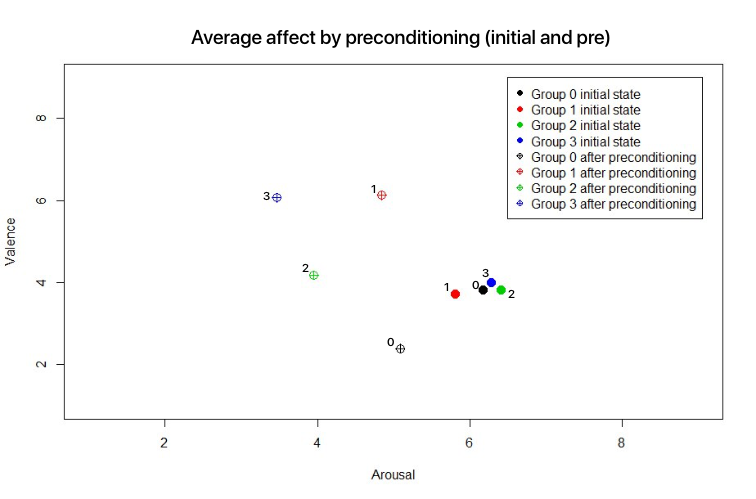
\includegraphics[width=1\linewidth]{graphics/after-preconditioning-avg}
	\caption[Avg Affect]{Average affect values before and after preconditioning}
	\label{fig:after-preconditioning-avg}
\end{figure}
		
		 As there is noticeable dispersion with the standard deviation of at least 1.19 points, I expect to see some participants not falling in the quadrant according to the preconditioning. A closer look is provided by the cross-table of \textit{quadrant-pre} variable and \textit{preconditioning} variable shown in Figure \ref{fig:preconditioningsuccessbygender}. The table shows participants, who have rated themselves in the target affect quadrant after preconditioning highlighted in green (or light-gray), and participants, who have rated themselves to be in one of the other quadrants. It is apparent that only about half of participants appear to be in the target quadrant. Despite this, the split is fairly equally distributed among four quadrants with the quadrant 1 being underrepresented, having only seventeen respondents.
		
\begin{figure}[h!]
	\centering
	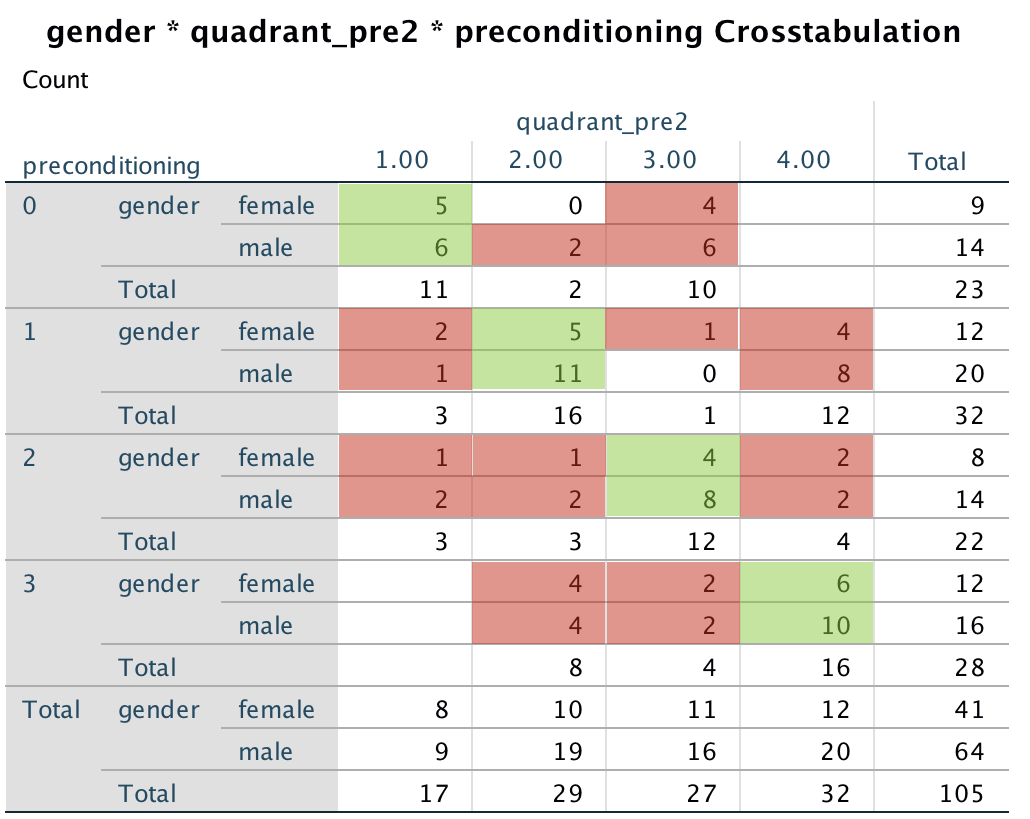
\includegraphics[width=0.7\linewidth]{graphics/preconditioning_success_by_gender}
	\caption{Affect quadrant by preconditioning group and gender}
	\label{fig:preconditioningsuccessbygender}
\end{figure}

		\subsubsection{Native speakers and E2 - creativity task} \label{sec:data-validity-native}
		
		During testing some feedback from participants included the difficulty of the creativity task (E2). Mostly this feedback has been from participants, who are non-native English speakers. This warrants a deeper look into data to see whether \textit{native} influences \textit{e2-total-points}. The null-hypothesis states:
		
		\textbf{H\textsubscript{0}:}  Native speakers (Question 3) do not score differently on the creativity task due to cultural influence 
		
		The difference between groups is assessed with a t-test run on 40 non-native speakers and 62 native speakers. A Welch t-test is run due to the assumption of homogeneity of variances being violated, as assessed by Levene's test for equality of variances (p = .003).
		Inspection of the box-plots indicates no outliers in the data. 
		\textit{e2-total-points} values are normally distributed for \textit{native} = 1 (p = .123), but not for \textit{native} = 0 (p = .029), as assessed by Shapiro-Wilk's test. 
		Native speakers score higher on the E2 test (M = 348.653, SD = 78.23732) compared to non-native speakers (M = 157.391, SD = 110.60). The difference is statistically significant with M = -191.26, 95\% CI [-231.44, -151.08], t(63.982) = -9.509, p < .001.
		
		I reject the null hypothesis of equality of means for native and non-native speakers. Native speakers score higher on the E2 test. This result is considered later during the analysis.


	\subsection{Analysis}
	
	Analysis of data is done with SPSS 25.
	
	\subsubsection{Hypothesis 1}
	
	As stated in Section \ref{sec:hypothesis} I analyze whether any effect on emotion can be attributed to the theme version. To validate this I look at valence and arousal values separately. The null hypotheses are stated as follows:
	
	\textbf{Null Hypothesis 1} H$_{01}$: There is no difference in \textbf{valence} between users of two different proposed interfaces.
	
	\textbf{Null Hypothesis 2} H$_{02}$: There is no difference in \textbf{arousal} between users of two different proposed interfaces.
	
	\paragraph{Data preparation and selection}
	
	To see the how arousal and valence change from SAM2 to SAM3 steps I compute 2 additional variables:
	
	\begin{enumerate}
		\item \textit{arousal-delta-2}: Change of arousal from SAM2 to SAM3
		\item \textit{valence-delta-2}: Change of valence from SAM2 to SAM3
	\end{enumerate}
	
	Apart from \textit{theme-version} other variables may contribute to a change of affect. These may include any performance metrics of the users during the task and the "enjoyment" factor of the task itself. As the tasks are the same for both theme versions the "enjoyment" parameter of the task is a controlled variable and can be neglected in the analysis.
	
	The performance metrics that are can be expected to influence the mood are specifically \textit{e1-pairs-opened} and \textit{e2-correct-guesses}. Two considerations are very important here: 1) Experiment 1 does not have a "lose" or "win" outcome definition and therefore each persons' own reflection on performance on the memory game is highly subjective. During on-site interviews after the task participants have shown bias towards assessing their performance on the memory game as subpar and much worse than potential other participants, regardless of their actual performance compared to others (which they were not informed about at the time). The effect on emotions from memory test maybe negatively skewed 2) Due to the recency effect, participants, when asked to evaluate their affect, can be heavily biased towards evaluation of their enjoyment of the second experiment (creativity test) as the main criterion for rating affect. The bias is evaluated below.
	
	\paragraph{Preparation: Relationship between e2-correct-guesses and affect values} 
	I assess the relationship between \textit{e2-correct-guesses} with \textit{valence-post} and \textit{arousal-post} respectively. 
	Visual inspection of a scatter-plot confirms some monotonic relationship for \textit{valence-post}, but not for \textit{arousal-post}.
	To assess this relationship a correlation test is conducted for \textit{valence-post} and \textit{arousal-post}.
	
	\begin{figure}
		\centering
		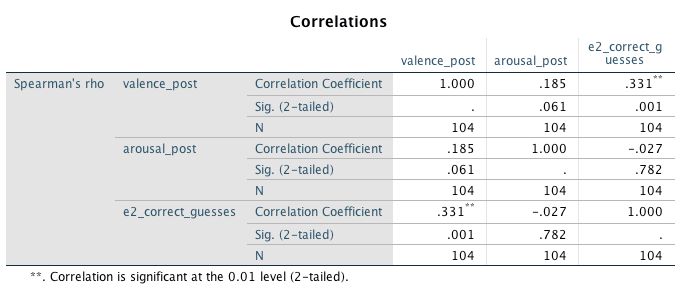
\includegraphics[width=1\linewidth]{graphics/correlationE2-correct-guesses-affect-post}
		\caption{Correlation test for valence-post, arousal-post, and e2-correct-guesses}
		\label{fig:correlatione2-correct-guesses-affect-post}
	\end{figure}
	
	One outlier (from mturk) with \(native = 1\) and \textit{e2-correct-guesses} = 0 is removed during data preparation under assumption, that they did not do the due diligence in solving the experiment questions. Normal distribution is not assumed for \textit{e2-correct-guesses} at this point. Spearman's rank-order correlation coefficient is used in lieu of Pearson correlation due to robustness towards non-normality of the former.
	
%	Several participants with e2-correct-guesses of 0 and 1 are also removed, due to possible general issues with the task. Further, participants with \textit{e1-pairs-opened} lower than 23 and higher than 95 are excluded as invalid. Overall 96 observations are kept as for this analysis.
	
	Results (illustrated in Figure \ref{fig:correlatione2-correct-guesses-affect-post} ) show that there is a statistically significant moderately strong positive correlation between \textit{valence-post} and \textit{e2-correct-guesses}, r\textsubscript{s} = .331, p < .001.
	
	No statistically significant correlation is found between \textit{e2-correct-guesses} and \textit{arousal-post}.
	
	\paragraph{Preparation: Variance of e2-correct-guesses by theme version}
	
	Because of the relationship between \textit{valence-post} and \textit{e2-correct-guesses}, an analysis of variance is beneficial for H$_{01}$. If the means between groups are equal then the factor \textit{e2-correct-guesses} will have a uniform impact on both groups of \textit{theme-version} in the subsequent analysis of variance for H$_{01}$ and H$_{02}$.
	
	Independent samples t-test is performed on the variable \textit{e2-correct-guesses} with a factor variable \textit{theme-version}, to assess whether there is a difference between means of the variable \textit{e2-correct-guesses} across theme versions. Absence of significant difference allows to move forward with the analysis of variance for H$_{01}$ and H$_{02}$.
	
	There are 52 participants with theme0, and 52 with theme1. The values do not show normal distribution per group as assessed by Q-Q Plots observation as well as Shapiro-Wilk test. The split between groups is equal and the skewness of distribution almost equal (-0.63 (SE -0.33) and -0.70 (SE -0.30)). The violation of normality is ignored in this case, as t-test can be considered robust against deviation from normality. The homogeneity of variances is confirmed, as assessed by Levene's test for equality of variances (p = 0.153). The t-test shows that the null hypothesis cannot be rejected and there is no statistically significant mean difference between the two groups (p = .714).
	
	For both theme versions the same distribution is observed on \textit{e2-correct-guesses}.
	
	
	\paragraph{H$_{01}$ Analysis of variance of \textit{valence-post} by theme and performance}
	
	I test whether there is an interaction effect between \textit{theme-version}, \textit{valence-pre}, and \textit{e2-correct-guesses} on the independent variable \textit{valence-post}.
	
	\textit{e1-pairs-opened} metric shows only extremely low correlation with both \textit{arousal-post} and \textit{valence-post} values and is excluded from the following analysis. The assumption here is that \textit{e1-pairs-opened} has no effect on affect values. Their perceived performance, if any, is overshadowed by the second task. As discussed earlier perceived performance for E1 task may be uniformly negative among participants as per their own self-evaluation. No question has been asked from participants about their perceived performance or enjoyment of the E1 task in the subsequent questionnaire.
	
	Metrics \textit{valence-pre}, and \textit{e2-correct-guesses} are continuous variables and for this test are transformed into categorical.
	\textit{valence-pre} is transformed into \textit{valence-group-pre} and split according to affect quadrant definition at the value \( V(pre) >= 5 \coloneqq 2; V(pre) < 5 \coloneqq 1\). \textit{e2-correct-guesses} \textit{e2-correct-guesses-grp} is split on the 50th percentile (at the value \(X >= 14 \coloneqq 2, X < 14 \coloneqq 1\))
	
	\begin{itemize}
		\item \textbf{Dependent:} \textit{valence-post}
		\item \textbf{Independent:} \textit{theme-version}, \textit{valence-group-pre}, \textit{e2-correct-guesses-grp}
	\end{itemize}
	
	A three-way ANOVA is conducted.
	Three outliers are removed, including two participants with extreme, almost unrealistic self-evaluation spread, and a participant, who did not solve any creativity task, despite being a native speaker (ID: IW3r*).
	Levene's test for equality of variances indicates homogeneity of variances for \textit{valence-post} for all group combinations (\(p = .079\)). 
	102 observations are included in the analysis. No statistically significant three-way interaction between \textit{theme-version, valence-group-pre and e2-correct-guesses-grp} could be observed, \(F(1, 94) = .161, p = .689\). Further, there is no statistically significant two-way interactions for each combination of these variables. (A problem could be due to samples size,  as graphical representation shows some possible interaction. Groups contain between 9 and 32 observations).
	
	It cannot be concluded that theme version has an effect on valence.
	
	\paragraph{H$_{02}$ Analysis of variance of \textit{arousal-post} by theme and performance}
	
	A similar procedure as above to assess an interaction effect between \textit{theme-version}, \textit{arousal-pre}, and \textit{e2-correct-guesses} on the independent variable \textit{arousal-post}. Categorical metrics derived in the previous analysis are used during this analysis again. Continuous variable \textit{arousal-pre} is transformed to categorical on the equivalent axis split as previous analysis into \textit{arousal-group-pre}
	
	\begin{itemize}
		\item \textbf{Dependent:} \textit{arousal-post}
		\item \textbf{Independent:} \textit{theme-version}, \textit{arousal-group-pre}, \textit{e2-correct-guesses-grp}
	\end{itemize}
	
	Categorical metrics derived in the previous analysis are used during this analysis again. A three-way ANOVA is conducted. Observations with (ID: IW3r*) and one outlier with extreme spread of ratings (possibly influenced by poor performance on the creativity task) is removed. No further outliers are present as per inspection of the box-plots.
	Shapiro-Wilk's test of normality shows three groups non-normally distributed (theme0, e2 perf - high, high arousal group, p = .027; theme1, low arousal group, both e2 perf groups with p = .005 and p = .018 for low and high respectively). Observation count is between 9 and 15 per group. Transformation attempts on the dependent variable did not yield a positive result for normality. I accept the violations of normality at this stage.
			      
	There is a statistically significant three-way interaction between \textit{theme-version}, \textit{arousal-group-pre}, and \textit{e2-correct-guesses-grp}, 
	F(1, 95) = 5.585, p = .020.
	
	According to this, simple two-way interaction between \textit{theme-version} * \textit{e2-correct-guesses-grp} based on each level of mediator variable \textit{arousal-group-pre} is assessed.
	
	There is a statistically significant simple two-way interaction between \textit{theme-version} and \textit{e2-correct-guesses-grp} for the high arousal group after preconditioning, \(F(1, 95) = 6.597, p = .012\), but not for low arousal group, \(F(1, 95) = .427, p = .515\).
	
	Statistical significance is shown on a $ p < 0.05 $, as well as on $ p < 0.025 $ level as per Bonferroni adjustment technique (with simple two-way interactions = 2).
	
	The analysis is followed up with simple simple main effects, with respect to: \textit{arousal-group-pre} $ = high $;
	
	There is a statistically significant simple simple main effect of \textit{theme-version} for high arousal-group-pre participants (i.e. participants getting the 0 or 1 preconditioning) at high amount of e2-correct-guesses (group 2), 
	$ F(1, 95) = 5.785, p < .018 $), 
	but no significant effect for high arousal-group-pre participants at low \textit{e2-correct-guesses-grp}, 
	$ F(1, 95) = 1.683, p = .198 $. 
	
	Table in Figure \ref{fig:h02-simple-simple-main-effects-test-results-table} shows the simple simple main effects and their significance. The significant main effect is highlighted in Figure \ref{fig:h02-simple-simple-main-effects-highlighted}.
	
	
\begin{figure}
	\centering
	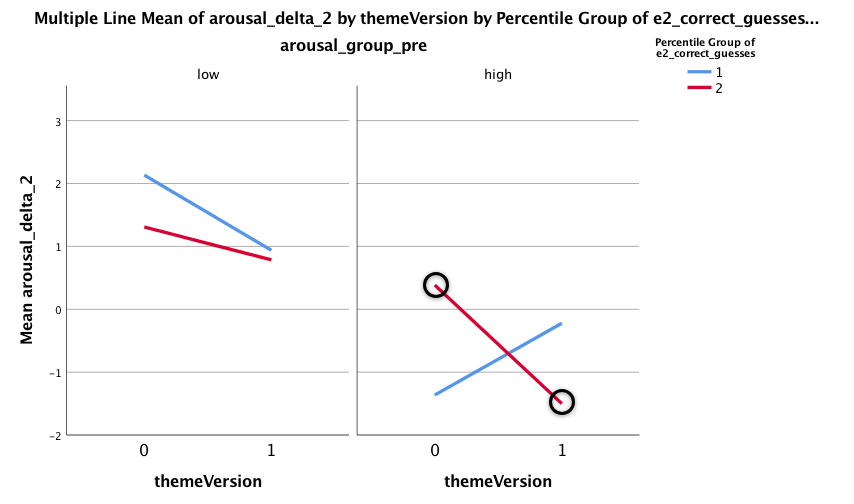
\includegraphics[width=1\linewidth]{graphics/H02-simple-simple-main-effects-highlighted}
	\caption{Significant simple simple main effects of the three-way-anova}
	\label{fig:h02-simple-simple-main-effects-highlighted}
\end{figure}
	
\begin{figure}
	\centering
	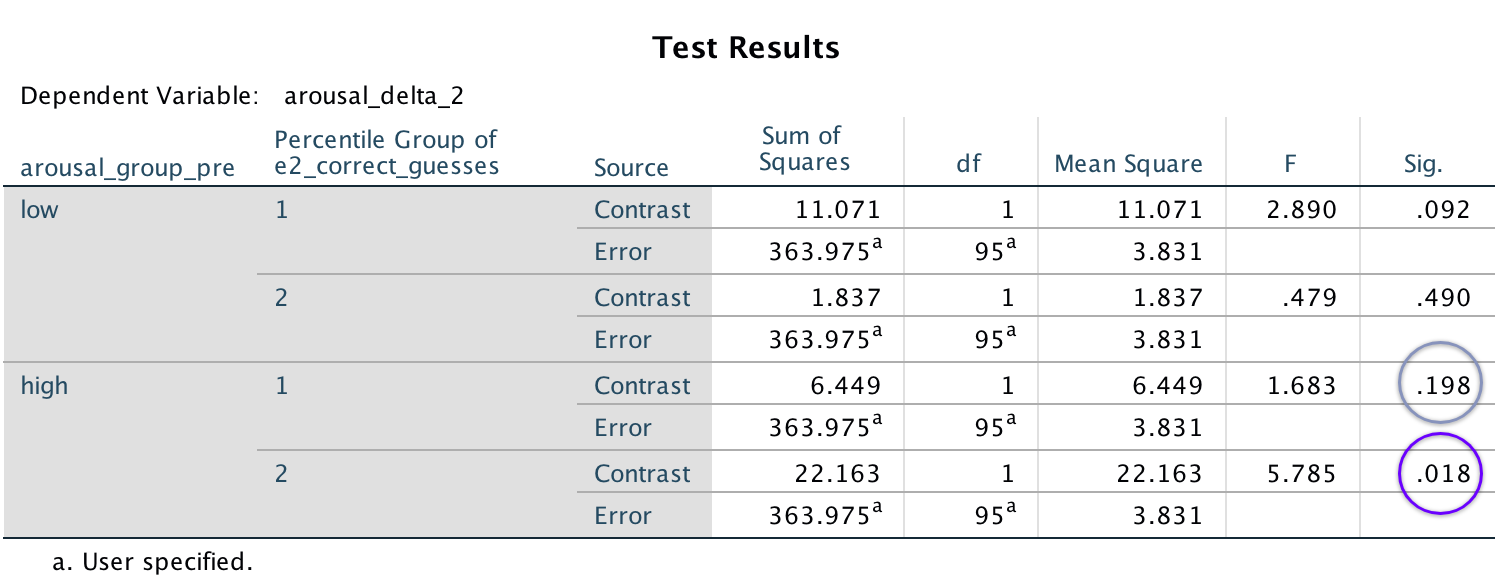
\includegraphics[width=1\linewidth]{graphics/H02-simple-simple-main-effects-test-results-table}
	\caption{Three-way ANOVA - simple simple main effects table}
	\label{fig:h02-simple-simple-main-effects-test-results-table}
\end{figure}

	For high arousal group with a high performance on E2 test simple simple main effect comparisons shows mean \textit{delta of arousal} for \textbf{theme0} is 0.385 of a point (SD = 0.543) and for \textbf{theme1} is -1.500 (SD = 0.565). The mean difference is statistically significant being 1.885 point, 95\% CI [0.329, 3.440], p = 0.018.
	
	\paragraph{Conclusion}
	
	No statistically significant difference of affect could be found for valence values across all groups. There is a statistically significant mean difference of arousal between theme versions for high performers of E2 when they are in angry or happy state (high arousal), whereas theme0 kept higher arousal for participants. Theme0 lowered the arousal values.
	
	\paragraph{Limitations} According to \cite{Russell2003} each persons average of affect values can vary. After an emotional episode each participant's emotions are bound to converge back to their default values with time. This process is not generalizable and should be accounted on a personal basis with further research. Due to current study design analysis is done with the assumption that each participants emotions behave in a similar way, despite evidence laid out by Russell.
	

%	- 1. compute delta of arousal and valence
%	- 2. remove outliers from 
%	e1-pairs-opened (the <= 22)
%	e2-total-points (none are outliers)
%	e2-correct-guesses (no outliers)
%	
%	- convert to categorical variable

	\subsubsection{Hypothesis 2: Introduction}

	With the Hypothesis 2 I analyze whether theme version has any effect on performance during experiment. Regardless, that no differences in the affect levels could be asserted with theme 1 compared to theme 0, it can be beneficial to check hypothesis 2 to uncover other potential effects on performance, perhaps caused on the subconscious level.
	
	Assertions made in hypothesis 2 can be separated in two parts, as the study design provides two types of separate experiments: memory and creativity. The following sections deal with each experiment separately.

	\subsubsection{Hypothesis 2: E1 Memory} \label{section:h2e1}
	
		I analyze whether theme version has any effect on performance during experiment 1 - Memory task.
		
		The null hypothesis \textbf{H$_{0}$:} Performance of participants on memory task, as measured by \textit{e1-pairs-opened}, is equal using theme 1 compared to using theme 0.
	
		\paragraph{Cleaning data} %\label{section:h2e1-cleaning}
		
		First, I check for irregularities with the data and outliers on the \textit{e1-pairs-opened}.
		
		A look at the data reveals, that some users have circumvented the memory game by making a screenshot of the open tiles, or, less probably, having perfect photographic memory. Figure \ref{tbl:e1-pairs-opened} shows the outliers highlighted. Due to this I exclude these respondents from the memory experiment analysis. Four of five participants in this group came from MTurk, one from social media.
		
		\begin{table}[]
			\begin{center}
				\begin{tabular}{|l|l|l|l|}
					\hline 
					source & gender & e1-total-duration-seconds & e1-pairs-opened \rule[-2ex]{0pt}{6ex} \\ \hline \hline
					turk   & male   & 104                          & \cellcolor[HTML]{FFFFC7}21                \\ \hline
					turk   & female & 86                           & \cellcolor[HTML]{FFFFC7}22                \\ \hline
					turk   & male   & 122                          & \cellcolor[HTML]{FFFFC7}22                \\ \hline
					turk   & male   & 90                           & \cellcolor[HTML]{FFFFC7}22                \\ \hline
					social & female & 185                          & \cellcolor[HTML]{FFFFC7}22                \\ \hline
					social & female & 218                          & 34                \\ \hline
				\end{tabular}
			\end{center}
			\caption{Memory outliers}
			\label{tbl:e1-pairs-opened}
		\end{table}
	
		An additional outlying data-point is revealed when looking at the overall duration of the memory game in seconds - \textit{e1-total-duration-seconds}. Respondent \#74 took several times longer than the nearest neighbor. Figure \ref{fig:memoryoutlier2} shows the box-plot distribution of the variable. Participant \#74 made a break during the test and is, therefore, also excluded. While total duration is not a performance metric as reasoned in section \ref{sec:e1metrics}, taking a break can be considered a strong mediating variable when dealing with short-term memory.
		
%		\begin{figure}
%			\centering
%			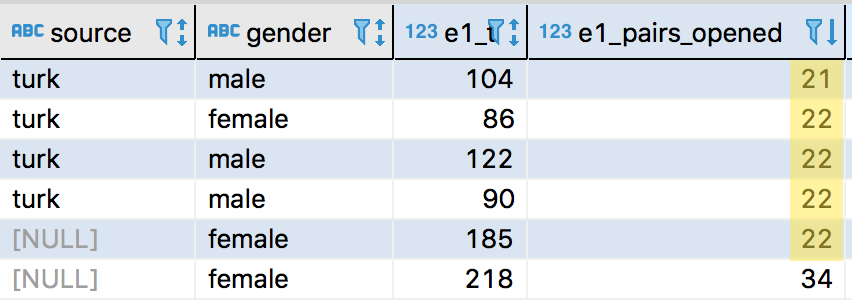
\includegraphics[width=0.7\linewidth]{graphics/MemoryOutlier1}
%			\caption{Memory outliers}
%			\label{fig:memoryoutlier1}
%		\end{figure}
		
		\begin{figure}
			\centering
			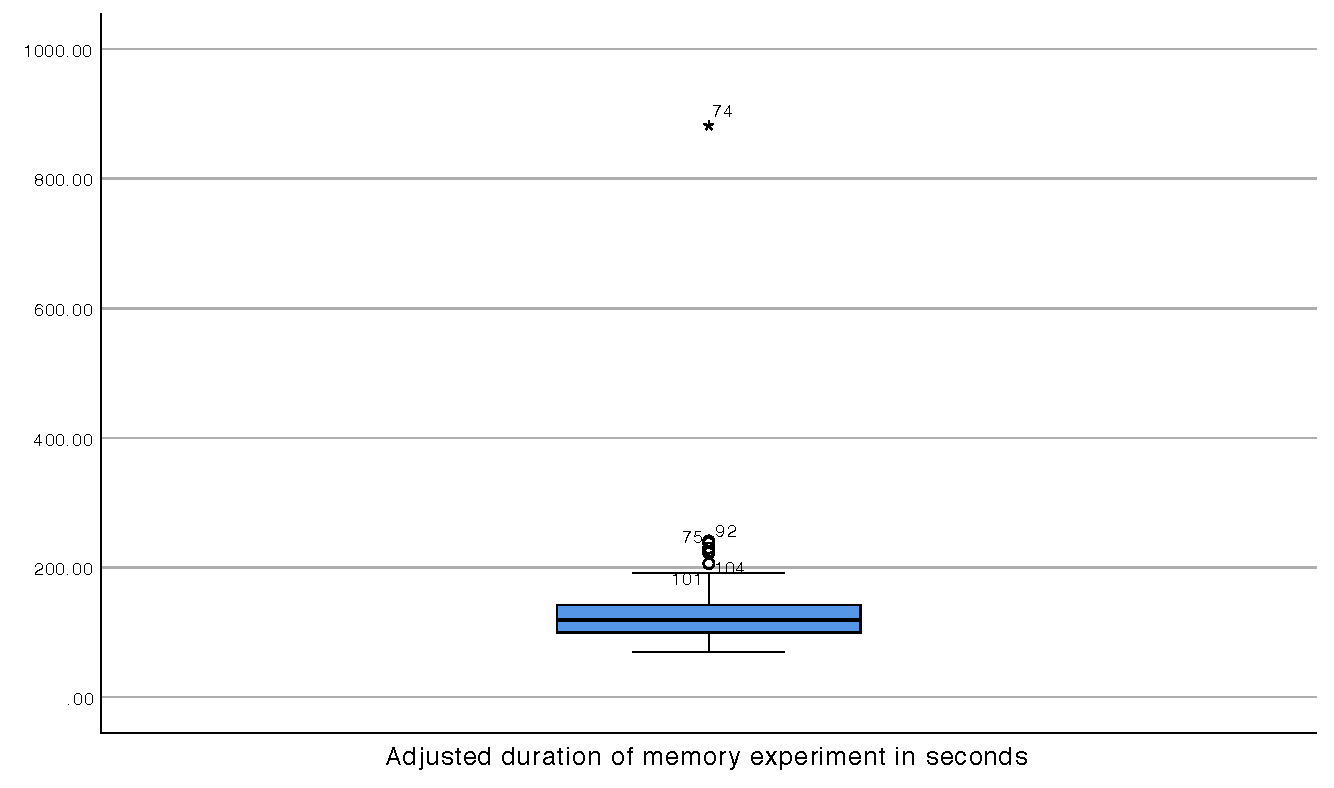
\includegraphics[width=0.7\linewidth]{graphics/memoryOutlier2}
			\caption{Memory duration outliers }
			\label{fig:memoryoutlier2}
		\end{figure}
	
		Table \ref{tbl:distribution} shows the distribution of people by affect quadrant group right after preconditioning step. 

		\begin{table}[h!]
			\centering
			\begin{tabular}{ll|l|llll|l}
				\hline
				\multicolumn{3}{l}{gender} & \multicolumn{4}{l}{quadrant-pre} & Total \\ \hline
				&              &   & 1.00    & 2.00   & 3.00   & 4.00   &       \\ \hline
				female  & themeVersion & 0 & 2       & 5      & 6      & 4      & 17    \\
				&              & 1 & 6       & 3      & 5      & 7      & 21    \\ \hline
				& Total        &   & 8       & 8      & 11     & 11     & 38    \\ \hline \hline
				male    & themeVersion & 0 & 4       & 13     & 6      & 9      & 32    \\
				&              & 1 & 5       & 5      & 7      & 11     & 28    \\ \hline
				& Total        &   & 9       & 18     & 13     & 20     & 60    \\ \hline \hline
				Total   & themeVersion & 0 & 6       & 18     & 12     & 13     & 49    \\
				&              & 1 & 11      & 8      & 12     & 18     & 49    \\ \hline \hline
				& Total        &   & 17      & 26     & 24     & 31     & 98 	\\ \hline \hline
			\end{tabular}
			\caption{Distribution of participants by theme, affect quadrant and gender}
			\label{tbl:distribution}
		\end{table}
		
		\paragraph{Preparation: Gender differences for E1}
		
		In a 1997 paper \cite{McBurney1997} suggests that some differences may be observed in the way male and female memory works.
		
		As I have unbalanced design with more male participants than female (see table \ref{tbl:distribution}), I assess whether women and men have significantly different memory test scores as measured by \textit{e1-pairs-opened}, and whether this can lead to a mediating effect on the performance across quadrants.
		
		Shapiro-Wilk test of normality rejects the null hypothesis of normal distribution. For this analysis I use the non-parametric Mann-Whitney U test, due to not normal distribution. Distributions of the scores for \textit{e1-pairs-opened} are similar for males and females, as assessed by visual inspection (both positively skewed). Median performance on the E1 task is not statistically significantly different between males (48.0) and females (49.0), $ U = 1099.500, z = -0.296, p = 0.768 $. Table \ref{tbl:e1means} shows median and mean values for \textit{e1-pairs-opened} across genders.
		
		\begin{table}[]
			\centering
			\begin{tabular}{l|l|l}
				Gender & Median & Mean       \\ \hline
				& e1-pairs-opened  & e1-pairs-opened		\\ \hline
				female & 49.00              & 50.18                 	 \\
				male   & 48.00              & 49.80                   	 \\ \hline
				Total  & 48.00              & 49.95                  	 \\ \hline \hline
			\end{tabular}
			\caption{Mean and Median values per gender for E1 metrics}
			\label{tbl:e1means}
		\end{table}
	
		As the test shows, that men and women do not have a difference in performance on the E1 task, I exclude this variable from further analysis as a mediating parameter.
		
		\paragraph{Analysis} 
		
		The present analysis tests the null hypothesis:
		
		\textbf{H$_{0}$:} Performance of participants on memory task, as measured by \textit{e1-pairs-opened}, is equal using theme 1 compared to using theme 0.
		
		With the outliers removed during data cleaning step, variable \textit{e1-pairs-opened} is factored by \textit{theme-version}. Shapiro-Wilk test of normality performed on the factored performance variable rejects the null hypothesis of normal distribution for both groups (theme0, p = 0.005; and theme1, p = 0.000).
		Some outliers are present in the higher value spectrum.
		
		\begin{figure}
			\centering
			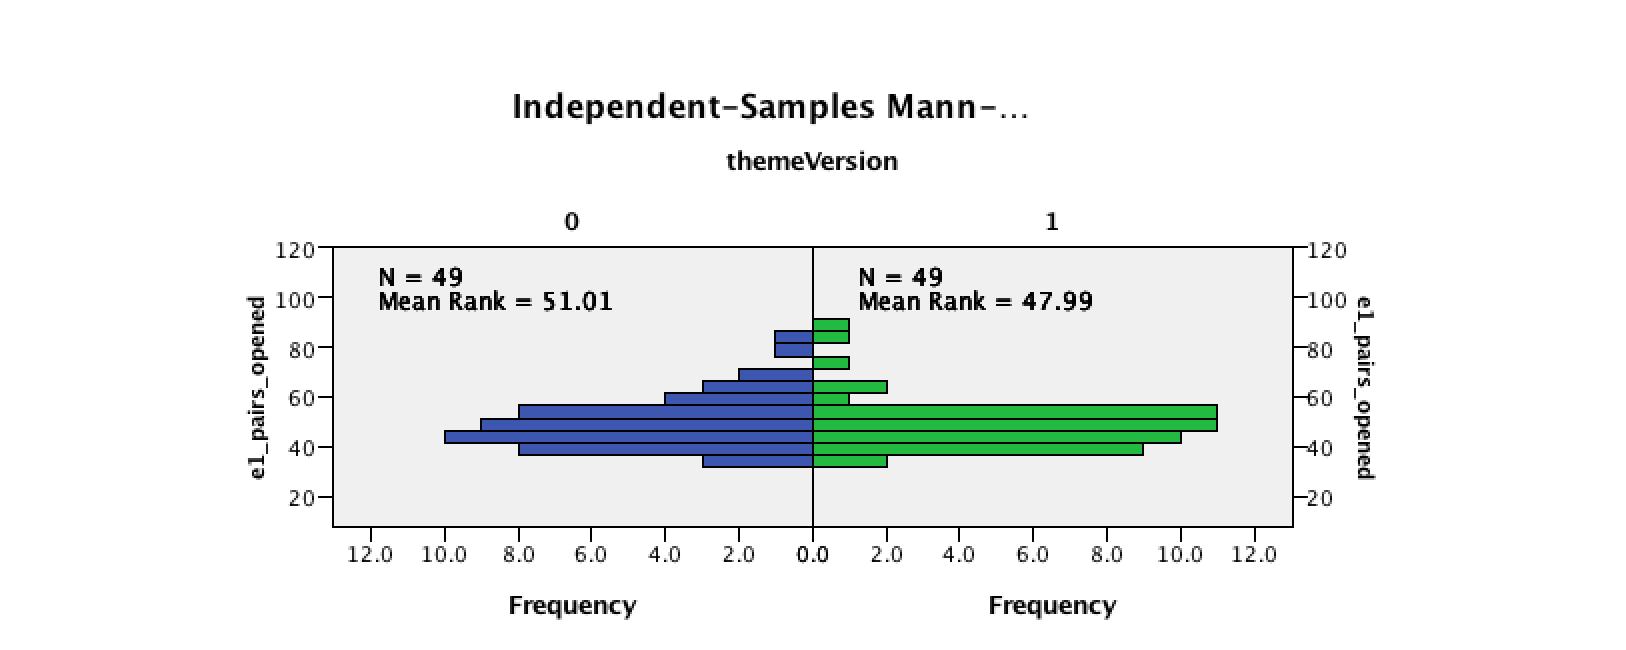
\includegraphics[width=1\linewidth]{graphics/H2E1-MannWhitneyU}
			\caption{Frequency graph of \textit{e1-pairs-opened} by theme version for Mann-Whitney U (Hypothesis 2, Experiment 1)}
			\label{fig:h2e1-mannwhitneyu}
		\end{figure}
		
		Due to outliers, a non-parametric Mann-Whitney U test is performed on the \textit{e1-pairs-opened} with the factor variable \textit{theme-version}. Distributions of the variable are similar for theme0 and theme1, as assessed by visual inspection of the frequency graphs (see Figure \ref{fig:h2e1-mannwhitneyu}). Median amount of pairs opened for theme0 (48) and theme1(48) are not statistically significantly different, U = 1126,5, z = -0.526, p = 0.599.
		
		An additional two-way ANOVA is performed to assess whether there is an interaction effect between \textit{quadrant-pre} and \textit{theme-version}. A range of outliers is, once again, present in the higher spectrum across groups, as assessed by box-plot observation. A two-way ANOVA is performed in two runs, once with outliers present (those described in paragraph on cleaning data in section \ref{section:h2e1} are still excluded, N = 98), and once with the most extreme outliers (2 outliers, N = 96) removed.
		
		For the analysis \textbf{with outliers present}, normality assumptions are violated for the residuals of two out of eight groups (as per Shapiro-Wilk test): 
		\begin{itemize*}
			\item theme = 1, quadrant-pre = 2 (p = 0.007, N = 8);
			\item theme = 1, quadrant-pre = 4 (p = 0.001, N = 18)
		\end{itemize*}. 
		There is homogeneity of variances, as assessed by Levene's test for equality of variances, $ p = 0.449 $.
		
		No statistically significant interaction is found for the two variables with outliers present: 
		$ F(3, 90) = 0.354, p = .787, \eta_{p}^{2} = .012 $.
		
		Followup analysis of main effects shows no statistically significant difference in E1 performance based on theme version ($ F(1, 90) = 0.011, p = .917, \eta_{p}^{2} = 0.00012. $), further it shows no statistically significant difference in E1 performance based on affect quadrant (defined by value of \textit{quadrant-pre}), ($ F(3, 90) = 0.374, p = .772, \eta_{p}^{2} = 0.012 $).
		
		%-------
		For the analysis \textbf{with outliers removed}, normality assumptions are not violated for the residuals (on a confidence level of p < 0.05) as per Shapiro-Wilk test. There is an observed homogeneity of variances, $ p = 0.130 $. Interaction effects are not significant, as assessed by two-way ANOVA. No followup analyses are done in this sub-test, as they are expected to yield comparable results.

		\begin{table}[]
			\centering
			\begin{tabular}{ll|l|ll}
				\hline
				\multicolumn{2}{l}{Descriptive Statistics}   &    & \multicolumn{2}{l}{e1-pairs-opened} \\ \hline
				theme-version          & quadrant-pre & N  & Mean          & Std. Deviation        \\ \hline
				0                      & 1.00         & 6  & 50.17         & 8.909                 \\
				& 2.00         & 18 & 51.17         & 10.788                \\ 
				& 3.00         & 14 & 51.21         & 17.480                \\ 
				& 4.00         & 14 & 50.57         & 13.727                \\ \hline
				1                      & 1.00         & 11 & 50.27         & 6.451                 \\
				& 2.00         & 11 & 43.64         & 19.038                \\ 
				& 3.00         & 13 & 49.31         & 12.828                \\ 
				& 4.00         & 18 & 46.50         & 11.526                \\ \hline
			\end{tabular}
			\caption{Descriptive Statistics for e1-pairs-opened}
			\label{tbl:group-sized-quadrant-theme-version}
		\end{table}
		
		Results of the analyses show that there are no statistically significant differences across groups of affect or theme versions for experiment 1. With collected information it cannot be determined whether observed outliers are due to people abusing the test or due to other reasons. Therefore, it is not considered safe to simply remove them, as they are believed to represent the population. Moreover, without them, the significance of the test improves only marginally, with no significant differences shown. A bigger sample is advised as some groups contain as little as six observations (see Table \ref{tbl:group-sized-quadrant-theme-version}). Differences, if any, are expected to be in lower percentage values and therefore a larger sample is advised for any significant result to manifest itself.
		
%		FR: Futher research: laboratory testing, more defined group of people, no above 45 people. Both genders can be tested, as there is not believed to be any effect of gender, although should be investigated in future research when applied.

	
	\subsubsection{Hypothesis 2: E2 Creativity}
	
	I analyze whether theme version has any effect on performance during experiment 2 - Creativity task.
	
	The null hypothesis \textbf{H$_{0}$:} Performance of participants on creativity task, as measured by \textit{e2-total-points}, is equal using theme 1 compared to using theme 0.
	
	\paragraph{Cleaning data}
	
%	Question 4 - proficiency. 
	
	Closer look at data shows that seven (7) participants assigned themselves to \textit{englishlevel} = 'Intermediate', all of whom are non-native speakers. Their mean \textit{e2-total-points} scores are also much lower as compared to native speakers. Level of English seems to correlate strongly with performance on the creativity task, regardless of native language. Figure \ref{tbl:stat-e2-total-points-by-lang} shows mean, std. error and median values per language group. As the question is asked right after completing the experiment, this measure can be subjective.
	
	\begin{table}[]
		\centering
		\begin{tabular}{ll|lll}
			\multicolumn{5}{l}{e2\_total\_points}                   \\ \hline
			native & englishlevel & Mean     & Std. Error & Median  \\ \hline
			0      & Intermed     & 84,7933  & 17,04154   & 71,252  \\
			& Advanced     & 140,259  & 21,20049   & 116,014 \\
			& Fluent       & 249,4089 & 38,45863   & 265,451 \\ \hline
			1      & Advanced     & 156,0835 & 81,6526    & 141,689 \\
			& Fluent       & 349,2958 & 10,21268   & 363,631 \\ \hline \hline
		\end{tabular}
		\caption{Descriptive Statistics for \textit{e2-total-points} by \textit{native} and \textit{englishlevel}}
		\label{tbl:stat-e2-total-points-by-lang}
	\end{table}

	Following analysis removes non-native users from consideration. As assessed in \ref{sec:data-validity-native}, only native speakers are expected to objectively show creativity differences without language skills being a mediating variable.

%	remove 7 people with intermediate skill, retain one person with beginner (deal as wrong entry)
	
	\paragraph{Preparation: Gender differences for E2}
	
	Similar to the test conducted for E1, I assess whether \textit{gender} has an effect on creativity task (E2) performance to control for a mediating effect of this variable.
	
	Data for both native and non-native is included in this test.
	Shapiro-Wilk test of normality rejects the null hypothesis of normal distribution. 
	Mann-Whitney U test is used to compare the groups of males and females. 
	Distributions of the values for \textit{e2-total-points} are similar for males and females, as assessed by visual inspection (both negatively skewed). 
	Median performance on the E2 task is not statistically significantly different between males (297.97) and females (296.39), $ U = 1194.500, z = -0.312, p = 0.755 $. 
%	Table \ref{tbl:e1means} shows median and mean values for \textit{e1-pairs-opened} across genders.
	
	As the test shows, that men and women do not have a difference in performance on the E2 task, I exclude this variable from further analysis as a mediating parameter for experiment 2.
	
	\paragraph{Analysis}
	
	The present analysis tests the null hypothesis:
	
	\textbf{H$_{0}$:} Performance of participants on memory task, as measured by \textit{e2-total-points}, is equal using interface 1 compared to using interface 0.
	
	With the outliers removed during data cleaning step, variable \textit{e2-total-points} is factored by \textit{theme-version}. The analysis is conducted over 62 participants with 33 using theme0 and 29 using theme1.
	Shapiro-Wilk test of normality performed on the factored performance variable retains the null hypothesis of normal distribution for theme0 (p = 0.785) and rejects it for theme1 (p = 0.039).
	One outlier is present for theme1 group with low performance (the participant has the highest amount of attempted guesses over the whole data-set, but only 7 out of 20 are correct).
	Due to the presence of an outlier, as well as non-normality of data Mann-Whitney U test is performed on \textit{e2-total-points} with the factor variable \textit{theme-version}. Distributions of the variable are similar for theme0 and theme1, as assessed by visual inspection (see Figure \ref{fig:h2e2-mannwhitneyu}). Median amount of pairs opened for theme0 (340.96) and theme1 (380.51) are not statistically significantly different, U = 526,0, z = 1.658, p = 0.097.
	
	\begin{figure}[h]
		\centering
		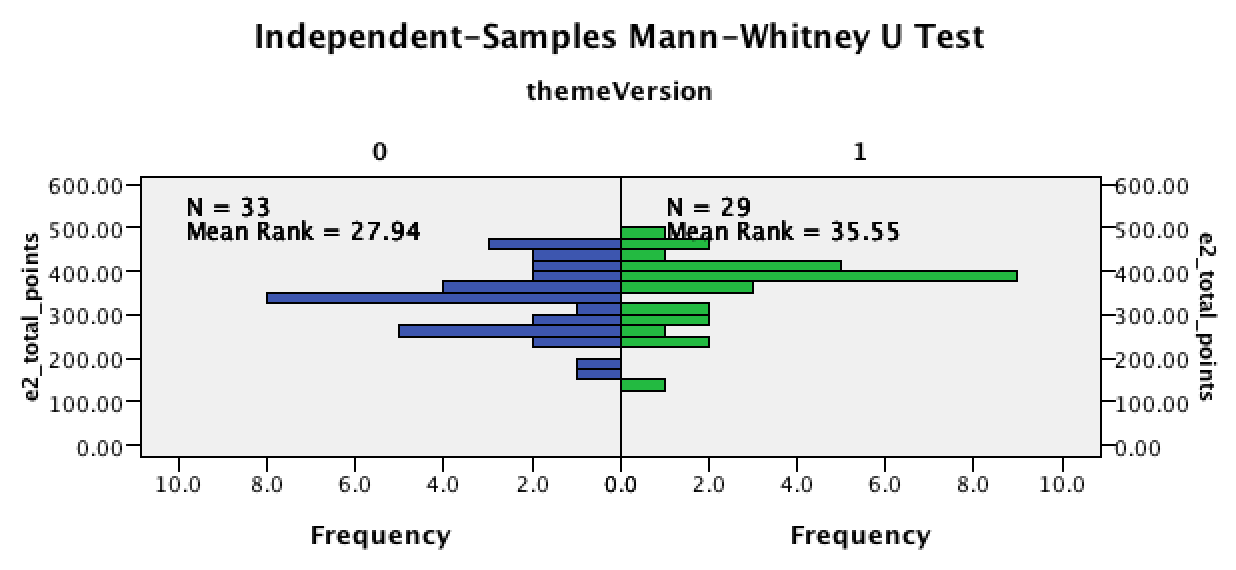
\includegraphics[width=0.8\linewidth]{graphics/H2E2-MannWhitneyU}
		\caption{Frequency graph of \textit{e2-total-points} by theme version for Mann-Whitney U (Hypothesis 2, Experiment 2)}
		\label{fig:h2e2-mannwhitneyu}
	\end{figure}
	
	An additional \textbf{two-way ANOVA} is performed to assess whether there is an interaction effect between \textit{quadrant-pre} and \textit{theme-version}, with \textit{e2-total-points} as dependent variable. Three outliers are present in the theme-version = 0, quadrant-pre = 3 group, in both high and low values, as assessed by inspection of the box-plot of the residuals. Other groups (7 groups) do not exhibit outliers. 
	
	\begin{table}[]
		\centering
		\begin{tabular}{ll|lll}
			\multicolumn{5}{l}{Dependent Variable:   e2-total-points}    \\
			theme-version & quadrant-pre & Mean     & Std. Deviation 			& N  \\ \hline
				0            & 1.00         & 383.1705 		& 41.53456       	& 4  \\
							& 2.00           & 336.8931 	& 60.08613       & 11 \\
							& 3.00           & 322.5621 	& 89.86881       & 9  \\
							& 4.00           & 328.2643 	& 99.16147       & 9  \\
							& Total          & 336.2407 	& 78.18744       & 33 \\ \hline
				1            & 1.00           & 366.1372 	& 60.54870       	& 6  \\
							& 2.00           & 388.2117 	& 55.41130       & 6  \\
							& 3.00           & 297.0977 	& 108.61095      & 7  \\
							& 4.00           & 391.4778 	& 47.19609       & 10 \\
							& Total          & 362.7778 	& 77.20360       & 29 \\ \hline
			Total        	& 1.00         	& 372.9505		 & 51.85708       	& 10 \\
							& 2.00           & 355.0055 	& 62.08867       & 17 \\
							& 3.00           & 311.4214 	& 95.89664       & 16 \\
							& 4.00           & 361.5346 	& 80.84257       & 19 \\
							& Total          & 348.6532 	& 78.23732       & 62
		\end{tabular}
		\caption{Descriptives for \textit{e2-total-points}}
		\label{tbl:h2e2-descriptives}
	\end{table}

	For the analysis \textbf{with outliers present}, all groups are normally distributed as per Shapiro-Wilk test (p > 0.05), The assumption of homogeneity of variances is violated, as assessed by Levene's test for equality of variances, p = .042. Transformation (squared transformation) of the variable \textit{e2-total-points} helps achieve homogeneity (p = 0.157), with the drawback of causing more outliers in the residual groups. Transformation is omitted in favor of preserving less outliers.
	
	No statistically significant interaction is found for the two variables with outliers present: $ F (3, 54) = 1.389, p = .256, \eta_{p}^{2} = .072 $.
	
	Followup analysis of main effects shows 
	no statistically significant difference in E2 performance based on theme version ($ F(1, 54) = 0.796, p = .376, \eta_{p}^{2} = 0.015 $), additionally it shows no statistically significant difference in E2 performance based on affect quadrant (defined by value of \textit{quadrant-pre}), ($ F(3, 54) = 2.07, p = .115, \eta_{p}^{2} = 0.103 $).
	
	For the analysis \textbf{with outliers removed},
	normality assumptions are not violated for the residuals (on a confidence level of p < 0.05) as per Shapiro-Wilk test. Homogeneity of variances is violated at $ p = 0.003 $. Interaction effects are not significant, as assessed by two-way ANOVA at $ p = 0.310 $. 
	%No followup analyses are done in this sub-test, as they are expected to yield comparable results.
	
	Followup analysis of main effects shows again
	no statistically significant difference in E2 performance based on theme version ($ F(1, 51) = 1.259, p = .267, \eta_{p}^{2} = 0.024 $), additionally it shows no statistically significant difference in E2 performance based on affect quadrant (defined by value of \textit{quadrant-pre}), ($ F(3, 51) = 2.642, p = .059, \eta_{p}^{2} = 0.134 $).
	
	While the effect of affect quadrant during creativity test performance is close to a significant result, it must be highlighted that the number of observations in this test was particularly low (see table \ref{tbl:h2e2-descriptives}). Had the result been significant it would suggest a lower performance for Q3 - sad, compared to all other quadrants.
	
	% Pairwise comparisons
	%\begin{figure}
	%	\centering
	%	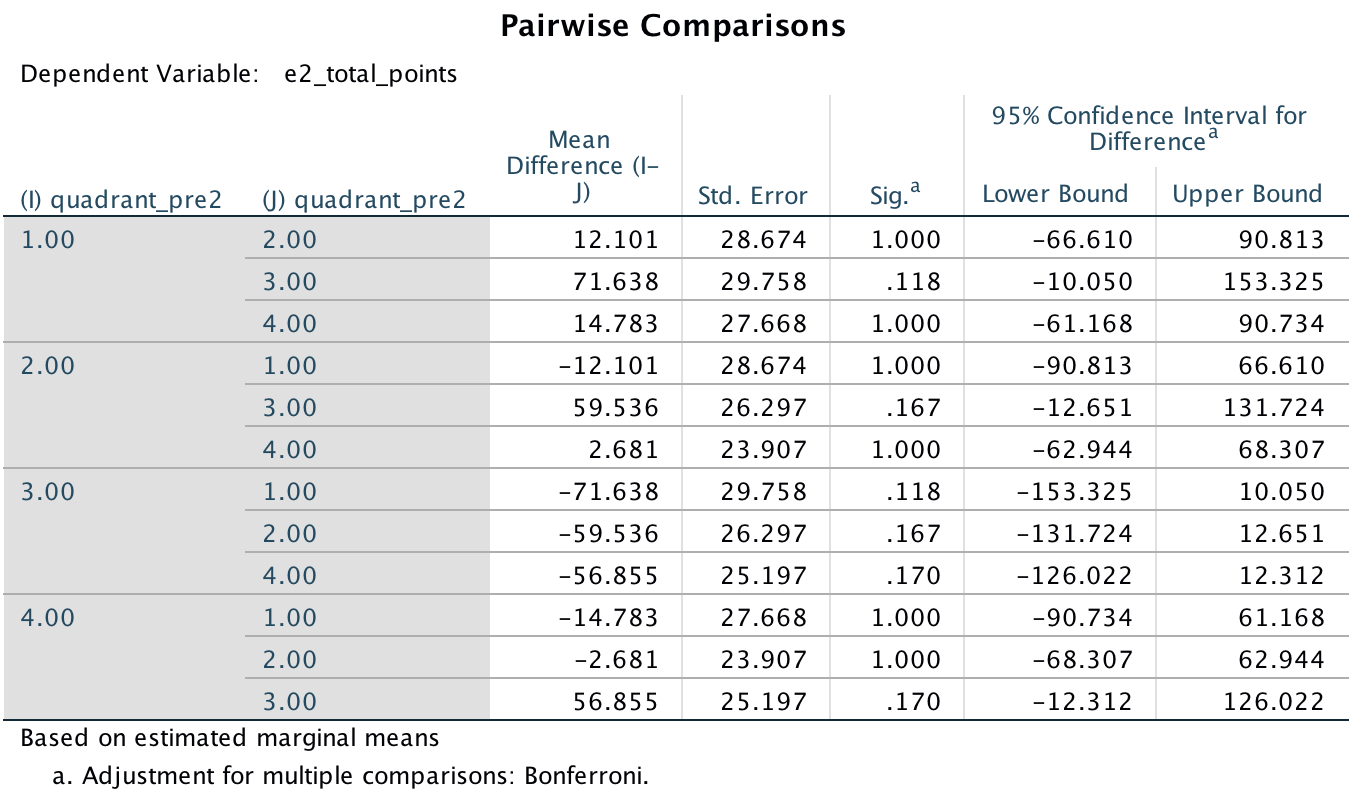
\includegraphics[width=0.7\linewidth]{graphics/pairwise-for-h2e2}
	%	\caption{}
	%	\label{fig:pairwise-for-h2e2}
	%\end{figure}
	
	Unfortunately at this sample size, as displayed in Table \ref{tbl:h2e2-descriptives} no statistically valid result can be concluded, and even though data shows some hints that are in line with past research and my assumptions before the study, statistical test assumptions during this analysis have been violated and any result should be taken with caution. Considerations for further research in regards to this hypothesis are discussed later in section \ref{sec:further-research}.
	
\section{Conclusions and Discussion}

	\subsection{Hypothesis 1}
	
	[Note:] H1 should be checked in the context of the whole app
	
	\subsection{Hypothesis 2}
	
	[Note:] H2 should be checked for each task separately
	
	\subsection{Limitations}
	
	\paragraph{Independence of the dimensions of Model of Affect}
	
	Current study assumption of the independence of the emotional axis of the circumplex model of affect can be set into doubt. A neuroscience study \cite{Bestelmeyer2017} analyzing brain signal activation levels suggest an interdependent relationship between pleasure and arousal emotions. 
	This would effectively suggest that induction of emotional state as attempted in this study with emotional stimuli is not easily attainable and some unknown mediating factors are at play. Interdependence of the two dimensions of arousal and valence is suggested by the U-shaped emotional stimuli distribution across several databases of emotional stimuli. There is some evidence that user's ratings of their emotional state does not reflect the reality, but rather reflects subjective assessment of momentary bursts of emotion and semantic "feeling" about the presented stimuli, rather than their actual effect on affect. Video based stimuli appear to be more potent in causing affect, yet require more technological consideration when used in research studies due to sound, bandwidth, as well as screen parameters.
	
	\paragraph{RAT inaccuracies}
	
	One of the problems presented in the Remote Associate Test yielded significantly lower correct answers than others with just 12\% guess rate compared to the average of 61\%. While it is unclear which word participants have been attempting exactly, there have been found at least one other word that fits the parameters.
%	SCHOOL VS COURT conundrum. People can guess court rather than school because it also fits .
	
	Another problem with the same test revolves around local expressions. While an effort has been made to clear problems from any words that are colloquial and local in nature, there have been reports among native English speakers from UK stating that a certain problem answer only exists as an expression in USA, but not in UK.	%EIGHTBALL is USA local
	
	Extensive feedback has been received during the conducting of the testing phase of the experiment. Participants, who are not English native speakers reported not being able to solve the problems effectively, and while they knew the words once answers appears, there was a lack of 'a-ha' effect and a general frustration with inability to find the answers. This outcome shows that RAT problems are heavily biased towards native speakers even though the words themselves are known to people they are not used in the daily lives of people and therefore are not salient in memory. \cite{Landmann2014} has proposed a German set of RAT problems developed for German native speakers. In the context of this study they would not be comparable to english language problems and could not have been used.
	
	Furthermore, it is possible that frustration at not answering the words and having to wait thirty seconds to receive the answer could skew the performance further into negative and affect results of the emotional questionnaire. Some form of frustration has been reported on several accounts during the study.
	
%reported feedback that creativity words are not known to non-natives, frustration and anger during creativity task. Skews results?

	\paragraph{General phrasing and language issues}
	
	Some participants reported struggling with the term "valence" during the emotional questionnaire. Having displayed the two extremes as "Negative" and "Positive" as well as the SAM pictorial guidance were not sufficient. The term has been considered to be replaced with "pleasure" during the course of the study phase. Although, due to danger of skewing the results, it has not been implemented.
	

		
	 \paragraph{Sample size} is at 105 participants. Although the distributions are healthy it is not possible to factor data by many parameters due to low statistical significance, as the resulting groups would have each just a few observations.
	\toDo{write}
	
	
	
	An additional question that can be asked is "how much did you enjoy this task" after each experiment to acquire their enjoyment factor.
	
	

\section{Further research} \label{sec:further-research}

\paragraph{Emotional affect model} The present research uses a two-dimensional representation of affect. A deeper understanding of effects can be achieved through adding the third dimension of \textit{dominance}. Alternatively describing more domain specific emotions can target more specific conclusions based on the e-learning domain, as proposed by \cite{SreejaPSMahalakshmi2017} and discussed in section \ref{sec:emotion-theory}.

\paragraph{Scope and sample size}
One difficulty that has been a recurring problem in this study is the large amount of groups and variables, both accounted for and unaccounted for (out of scope), these variables create a fragmentation of data, leaving each group with only few participants. At this point the study becomes much less reliable. Differences between groups can sometimes be minimal and can be obfuscated behind regular variances between study subjects. For this type of study a much higher sample size is needed.

\paragraph{Study design} As a measure to combat low sample size it is possible to use the within-subjects design approach. The same participant would, over a period of time, accomplish the same task and exposed to different preconditioning. This is possible with the memory task used in current research. Creativity task (Remote associate) is not compatible with within-subjects design (further discussed below).

\paragraph{Improving E2 Creativity test design}
During current study I has been uncovered that there is a lacking degree of applicability of the Remote Associates Test on non-native speakers. As such, future research should control for native speakers only in the study design. Additionally there is a variability of creative thinking per person, whereas some participants might show higher scores than others with the same preconditioning and affect values. A within-subject design can be considered to control for variation of intrinsic characteristics of a person. Such design can be limited since, remote associate problems can be solved only once (being know to the participant later) and they are not readily comparable among each other to be able to mix different RAT-sets between studies. Alternatively, a large enough sample size could reduce this effect, at which point one could imply a random distribution of creative ability at each group.

\paragraph{Effect of preconditioning}

Nowadays, people are exposed to emotional stimuli often. Both strong and otherwise. This can lead to certain stimuli losing their effectiveness. For example, a person which is regularly exposed to a specific stimuli in their daily life due to the effect of habituation, would not respond to it as strongly, as someone experiencing it for the first time. When choosing participant groups, more focus can be provided to having a uniform background among them, thereby controlling for the aforementioned effects.

\paragraph{Emotional affect rating}
Study design in this case opts for using SAM (see section \ref{sec:selfeval}) as a means to rate affect level. During the study reports and observations showed that some participants can have problems evaluating the questions. As such, the word \textit{arousal}, to some, can imply colloquial meaning that is not the intention in this context. Further, participants can be "compelled" to rate their affect levels by what they feel they should feel, rather than what they actually feel. This can lead to subjective ratings.
Usage of implicit questions, where the mapping is not readily clear between the image and the (expected) response, could show more realistic results for affect ratings (section \ref{sec:selfeval}).

\paragraph{Design features}
Current implementation of the emotional design features limits these to only few parameters. A stronger differentiation and longer, more realistic exposure to an interface that more highly resemble an online learning interface may lead to more strongly defined response.

\paragraph{Global theme definition in emotionally aware interfaces}
The idea of an interface that can judge which task is more supported by which interface and emotional state is based on the prerequisite that emotional state and interface are variables that influence learning. Current research has not shown consistent response patterns of such relationship. In this respect a global theme definition cannot argued to have a use-case in this context. However, a similar architectural pattern can be introduced into the learning environment to facilitate smarter guidance of lessons. For example users can make choices during the course of their learning. These choices can then be used to form a user model and guide an adaptive interface to produce the most fitting lesson format for the user.
A rudimentary example sees the system learning which format the user prefers to learn with (i.e. video, text, graphical, acoustical). Later the system makes decisions for the user based on previous choices and context.
%- Additional benefits of global theme definition in the context of an emotionally aware interface?

%- limit variables and insrease sample size



\section{Ethical, legal and social implications}

[TODO]

\section{Notes}

\begin{figure}[ht!]
	\centering
	\begin{minipage}{.4\textwidth}
		\centering
		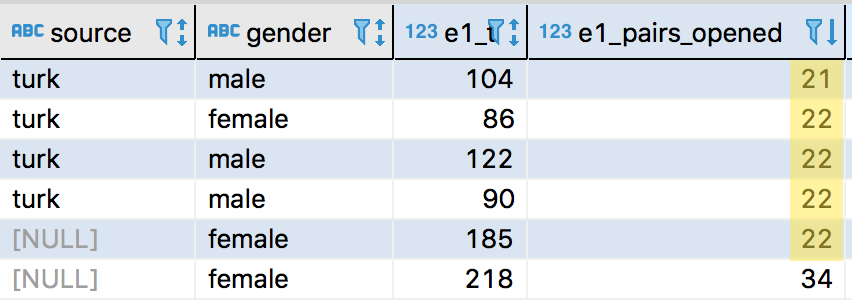
\includegraphics[width=1\linewidth]{graphics/MemoryOutlier1}
		\captionof{figure}{A figure}
		\label{fig:test1}
	\end{minipage}%
	\begin{minipage}{.6\textwidth}
		\centering
		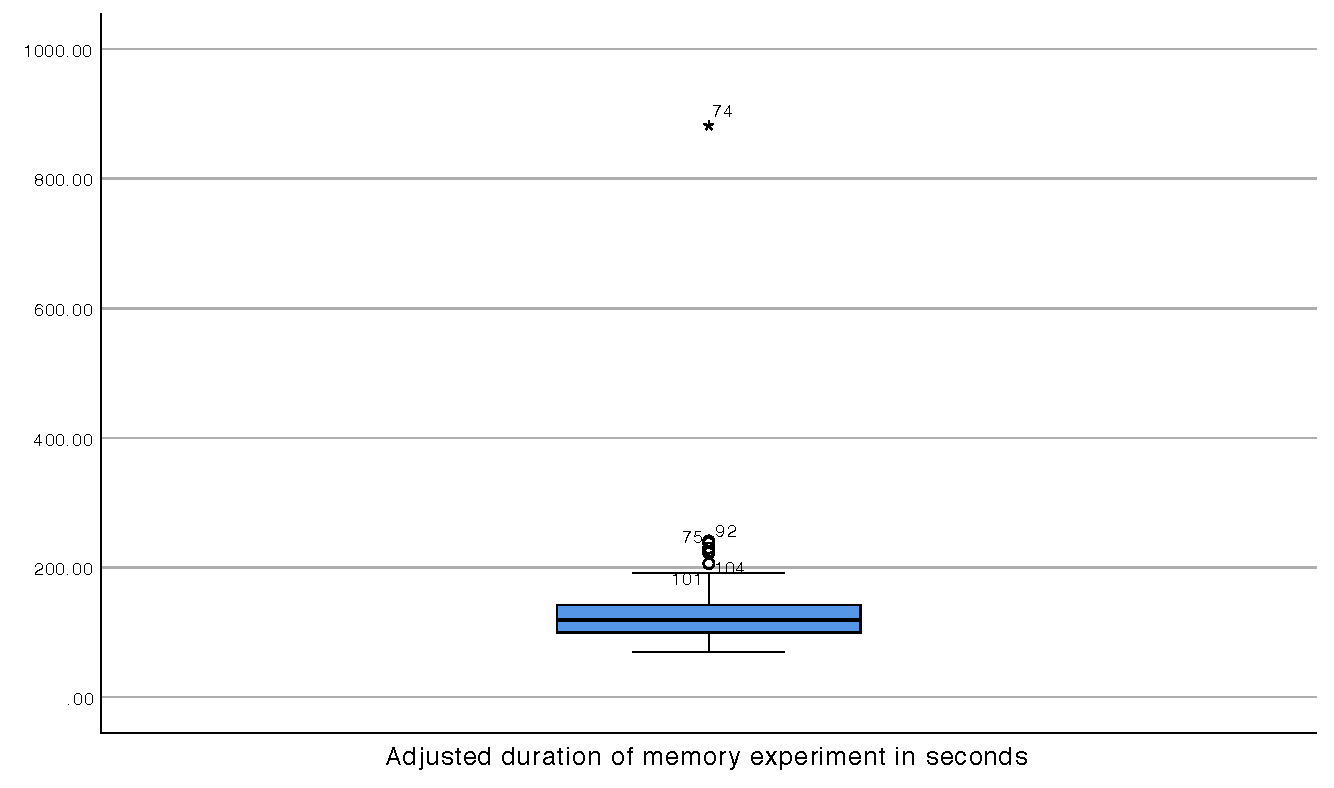
\includegraphics[width=1\linewidth]{graphics/memoryOutlier2}
		\captionof{figure}{Another figure}
		\label{fig:test2}
	\end{minipage}
\end{figure}



